\chapter{自旋}\label{chp:07}
% \makebox[5em][s]{} % 短题目拉间距

% 电子自旋
\section[电子自旋]{电子自旋} \label{sec:07.01} % 
% \makebox[5em][s]{} % 短题目拉间距

{\heiti 1. 自旋的基本性质}

自旋角动量和自旋磁矩是基本粒子的一种内禀属性,已经为许多直接与间接的实验所证实.1925年,基于碱金属光谱的双线结构和反常塞曼效应等实验事实,乌伦贝克与高德斯密特提出了电子具有自转的假设,“自旋” 这名词即由此而来.

现在,关于电子自旋已经确定下列实验事实:

(i) 自旋角动量在任何方向的投影只能取量子化数值$\pm\frac{\hbar}{2}$.

(ii) $\frac{\text{自旋磁矩}}{\text{自旋角动量}}=\frac{-e}{m_{e}c}$$\bigg[$作为对比,电子的轨道磁矩与轨道角动量的比值为$\frac{-e}{2m_{e}c}$	.$\bigg]$

将电子自旋简单地理解成自转是不妥当的,理由如下.如将电子当作半径为$\boldsymbol{r}$的小球,如电子由于自转而造成数值达$\frac{\hbar}{2}$的角动量,则其表面转速将达$v\sim\frac{\hbar}{rm_{e}}$,由于$r<10^{-3}\si{fm}$,
\eqllong
\begin{empheq}{equation*}
	v\sim\frac{\hbar}{rm_{e}}=\frac{\hbar c^{2}}{rm_{e}c^{2}}>c\times\frac{200\si{MeV}\cdots\si{fm}}{10^{-3}\si{fm}\times0.5\si{MeV}}\approx c\times 4\times 10^{5}
\end{empheq}\eqnormal
$v$远超过光速,这是违反狭义相对论的.另外,中子无电荷,但仍具有自旋磁矩,这就更难给予形象化的解释了.

现在比较公认的看法是,“自旋”是基本粒子的固有内禀属性(正如质量和电荷是内禀属性),其来源尚不清楚,但性质(量纲)类似于轨道角动量与轨道磁矩,并可以互相耦合.在研究电子的运动状态时,应该将自旋作为一种内禀(独立于空间“轨道”运动)自由度.

质子和中子也都有自旋.它们的自旋角动量在任何方向的投影,与电子一样,只取量子化数值$\pm\frac{\hbar}{2}$.自旋磁矩(投影)的数值也是量子化的,但和电子相比,质子与中子的自旋磁矩显得有些“反常”.如前所述,电子自旋磁矩(投影)取值为$\mp\mu_{B}$,$\mu_{B}$为玻尔磁子,即
\eqshort
\begin{empheq}{equation*}
	\mu_{B}=\frac{e\hbar}{2m_{e}c}
\end{empheq}\eqnormal
测量核子磁矩,通常以核磁子$\mu_{N}\frac{e\hbar}{2m_{p}c}$为标准,质子和中子的自旋磁矩(投影)分别为
\begin{empheq}{equation*}
	\mu_{p}=\pm\num{2.793}\mu_{N},\quad \mu_{n}=\mp\num{1.913}\mu_{N}
\end{empheq}

{\heiti 2. 自旋算符与自旋波函数}

以$\boldsymbol{S}$表示电子自旋角动量算符,假设其分量$S_{x},S_{y},S_{z}$都是厄密的($S_{x}^{+}=S_{x}$,等等),而且满足与轨道角动量一样的对易式,即
\begin{empheq}{equation}\label{eq71.1}
	S_{x}S_{y}-S_{y}S_{x}=i\hbar S_{z},\text{等等}
\end{empheq}
亦即
\eqshort
\begin{empheq}{equation*}\label{eq71.1'}
	S\times S=i\hbar S	\tag{$7.1.1^{\prime}$}
\end{empheq}\eqnormal
这样假设的理由是,$\S$\ref{sec:04.07}曾从这种对易式出发,导出角动量(平方及投影)的本征值,其中$j=\frac{1}{2}$的情况刚好和电子自旋相符合.

根据实验测量,$S$在任何方向的投影的取值只能是$\pm\frac{\hbar}{2}$,因此成立下列算符关系:
\begin{empheq}{align}	%2,3
	&S_{x}^{2}=S_{y}^{2}=S_{z}^{2}=\frac{\hbar^{2}}{4}		\label{eq71.2}\\
	S^{2}&=S_{x}^{2}+S_{y}^{2}+S_{z}^{2}=\frac{3\hbar^{2}}{4}		\label{eq71.3}
\end{empheq}
\eqref{eq71.1}至\eqref{eq71.3}式包括了电子自旋角动量的全部性质,其中\eqref{eq71.1}式是任何角动量的共性,\eqref{eq71.2}、\eqref{eq71.3}式则是电子自旋特有的.

为了简化运算,引入无量纲的“泡利自旋算符”$\boldsymbol{\sigma}$,
\eqshort
\begin{empheq}{equation}\label{eq71.4}
	S=\frac{\hbar}{2}\boldsymbol{\sigma}
\end{empheq}\eqnormal
则\eqref{eq71.1}式变成
\begin{empheq}{equation}\label{eq71.5}
	\sigma_{x}\sigma_{y}-\sigma_{y}\sigma_{x}=2i\sigma_{z},\text{等等}
\end{empheq}
亦即
\eqshort
\begin{empheq}{equation*}\label{eq71.5'}
	\boldsymbol{\sigma}\times\boldsymbol{\sigma}=2i\boldsymbol{\sigma}		\tag{$7.1.5^{\prime}$}
\end{empheq}\eqnormal
\eqref{eq71.2}式变成
\begin{empheq}{equation}\label{eq71.6}
	\sigma_{x}^{2}=\sigma_{y}^{2}=\sigma_{z}^{2}=1
\end{empheq}
\eqref{eq71.3}式变成
\begin{empheq}{equation}\label{eq71.7}
	\boldsymbol{\sigma}^{2}=\sigma_{x}^{2}+\sigma_{y}^{2}+\sigma_{z}^{2}=3
\end{empheq}
以$\sigma_{x}$分别从右和从左乘\eqref{eq71.5}式,再利用\eqref{eq71.6}式,易得
\eqindent{12}
\begin{empheq}{equation}\label{eq71.8}
	\sigma_{z}\sigma_{x}=-\sigma_{x}\sigma_{z}
\end{empheq}
类似地可证
\begin{empheq}{equation*}\label{eq71.8'}
	\begin{aligned}
		\sigma_{x}\sigma_{y}=-\sigma_{y}\sigma_{x}	\\
		\sigma_{y}\sigma_{z}=-\sigma_{z}\sigma_{y}
	\end{aligned}	\tag{$7.1.8^{\prime}$}
\end{empheq}
以\eqref{eq71.8'}代入\eqref{eq71.5}式,即得
\begin{empheq}{equation}\label{eq71.9}
	\sigma_{x}\sigma_{y}=i\sigma_{z},\text{等等}
\end{empheq}\eqnormal
\eqref{eq71.6}、\eqref{eq71.8}、\eqref{eq71.9}式可以统一成一个公式
\begin{empheq}{equation}\label{eq71.10}
	\boxed{\sigma_{\alpha}\sigma_{\beta}=\delta_{\alpha\beta}+i\sum_{\gamma}\varepsilon_{\alpha\beta\gamma}\sigma_{\gamma}}
\end{empheq}
其中$\alpha,\beta,\gamma$各自代表$(x,y,z)$三个分量中任何一个,$\varepsilon_{\alpha\beta\gamma}$为Levi-Civita符号,定义为
\eqlong
\begin{empheq}{equation*}
	{\varepsilon_{\alpha\beta\gamma}=}
	\begin{dcases}
		0,\qquad	\alpha\beta\gamma\text{有相同者}	\\
		1,\qquad	(\alpha\beta\gamma)=(x,y,z),(y,z,x),(z,x,y)	\\
		-1,\quad	(\alpha\beta\gamma)=(x,z,y),(y,x,z),(z,y,x)
	\end{dcases}
\end{empheq}
[按惯例,\eqref{eq71.10}式中求和号$\sum_{\gamma}$常常略去不写.]\eqref{eq71.10}式概括了泡利自旋算符$\sigma$的全部代数性质.但此式初学者不易掌握,不如记住\eqref{eq71.6}至\eqref{eq71.9}式.

由于$S_{x},S_{y},S_{z}$互不对易,没有共同本征态,电子的自旋状态一般只能采用下述表述方式.任取$\boldsymbol{S}$的一个分量$S_{z}$,以它的本征态作为基本自旋函数,任何自旋态则表示成这些本征态的线性叠加.$S_{z}$取本征值$\frac{\hbar}{2}$时,本征态记为$\chi_{1/2}$或$\alpha$,本征值$(-\frac{\hbar}{2})$的本征态记为$\chi_{-1/2}$或$\beta$,即
\begin{empheq}{equation}\label{eq71.11}
	\begin{aligned}
		S_{z}\chi_{1/2}	&=\frac{\hbar}{2}\chi_{1/2}
		S_{z}\chi_{-1/2}&=-\frac{\hbar}{2}\chi_{-1/2}
	\end{aligned}
\end{empheq}\eqnormal
如以$\chi_{1/2},\chi_{-1/2}$作为自旋态矢空间的基矢,建立“$S_{z}$表象”,则这两个本征态表示成
\begin{empheq}{equation}\label{eq71.12}
	\chi_{1/2}=\begin{bmatrix}
		1 \\ 0
	\end{bmatrix},\quad \chi_{-1/2}=\begin{bmatrix}
		0 \\ 1
\end{bmatrix}
\end{empheq}
电子的任何自旋态$\chi$可以表示成
\begin{empheq}{equation}\label{eq71.13}
	\chi=C_{1}\chi_{1/2}+C_{2}\chi_{-1/2}=\begin{bmatrix}
		C_{1} \\ C_{2}
	\end{bmatrix}
\end{empheq}
这也就是以$S_{z}$作为自旋变量时自旋波函数的表示形式,所以\eqref{eq71.13}式左端也可写成$\chi(S_{z})$,$C_{1}$和$C_{2}$就是当$S_{z}$等于$\pm\frac{\hbar}{2}$时波函数$\chi$的值,$C_{1}$和$C_{2}$的概率含义则是
\begin{empheq}{align*}
	|C_{1}|^{2} &=\text{$\chi$态下$S_{z}$取值$\frac{\hbar}{2}$的概率}	\\
	|C_{2}|^{2} &=\text{$\chi$态下$S_{z}$取值$\bigg(-\frac{\hbar}{2}\bigg)$的概率}
\end{empheq}
当然,自旋波函数应该满足归一化条件
\eqlong
\begin{empheq}{equation}\label{eq71.14}
	\chi^{+}\chi=[C_{1}^{*}\quad C_{2}^{*}]\begin{bmatrix}
		C_{1} \\ C_{2}
	\end{bmatrix}=C_{1}^{*}C_{1}+C_{2}^{*}C_{2}=1
\end{empheq}\eqnormal

在$S_{z}$表象中,$\boldsymbol{S}$及$\boldsymbol{\sigma}$各分量应该表示成二阶厄密矩阵,其中$S_{z},\sigma_{z}$为对角矩阵,对角元等于本征值.因此可以直接写出
\begin{empheq}{equation}\label{eq71.15}
	S_{z}=\begin{bmatrix}
		\frac{\hbar}{2} & 0		\\
		0 & -\frac{\hbar}{2}	\\
	\end{bmatrix},\quad \sigma_{z}=\begin{bmatrix}
		1 & 0	\\
		0 & -1	\\
\end{bmatrix}
\end{empheq}
下面来确定$\sigma_{x}$和$\sigma_{y}$的矩阵表示.设
\begin{empheq}{equation*}
	\sigma_{x}=\begin{bmatrix}
		a & b	\\
		b^{*} & c	\\
	\end{bmatrix}\quad \text{($a,c$为实数,因为$\sigma_{x}=\sigma_{x}^{*}$)}
\end{empheq}
由\eqref{eq71.8}式,易得$a=c=0$,而由\eqref{eq71.6}式,又可得$b^{*}b=1$.至此已经没有公式可以利用了.作为一种简明的选择,取$b=1$,则
\eqshort
\begin{empheq}{equation*}
	\sigma_{x}=\begin{bmatrix}
		0 & 1 \\
		1 & 0 \\
	\end{bmatrix}
\end{empheq}\eqnormal
再利用\eqref{eq71.9}式$(\sigma_{z}\sigma_{x}=i\sigma_{y})$,即可定出$\sigma_{y}$.总的结果是
\eqllong
\begin{empheq}[box=\widefbox]{equation}\label{eq71.16}
	\sigma_{x}=\begin{bmatrix}
		0 & 1 \\
		1 & 0 \\
	\end{bmatrix},\sigma_{y}=\begin{bmatrix}
	0 & -i \\
	i & 0 \\
\end{bmatrix},\sigma_{z}=\begin{bmatrix}
1 & 0 \\
0 & -1 \\
\end{bmatrix}
\end{empheq}\eqnormal
这就是著名的泡利矩阵.容易验证,这三个矩阵满足\eqref{eq71.6}至\eqref{eq71.9}全部关系式.泡利矩阵对于$\chi_{1/2}$及$\chi_{-1/2}$的作用结果是
\eqlong
\begin{empheq}{equation}\label{eq71.17}
	\begin{aligned}
		&\sigma_{x}\chi_{1/2}=\chi_{-1/2},\quad  &\sigma_{x}\chi_{-1/2}=\chi_{1/2}	\\
		&\sigma_{y}\chi_{1/2}=i\chi_{-1/2},\quad &\sigma_{y}\chi_{-1/2}=-i\chi_{1/2}	\\
		&\sigma_{z}\chi_{1/2}=\chi_{1/2},\quad   &\sigma_{x}\chi_{-1/2}=-\chi_{1/2}
	\end{aligned}
\end{empheq}
因此
\begin{empheq}{equation}\label{eq71.18}
	\begin{aligned}
		&(\sigma_{x}+i\sigma_{y})\chi_{1/2}=0,\quad &(\sigma_{x}+i\sigma_{y})\chi_{-1/2}=2\chi_{1/2}	\\		
		&(\sigma_{x}-i\sigma_{y})\chi_{-1/2}=0,\quad &(\sigma_{x}-i\sigma_{y})\chi_{1/2}=2\chi_{-1/2}	
	\end{aligned}
\end{empheq}
如将$\boldsymbol{\sigma}$换成$\boldsymbol{S}$,\eqref{eq71.18}式就是
\begin{empheq}{equation}\label{eq71.19}
	\begin{aligned}
		&(S_{x}+iS_{y})\chi_{1/2}=0,\quad &(S_{x}+iS_{y})\chi_{-1/2}=\hbar\chi_{1/2}	\\		
		&(S_{x}-iS_{y})\chi_{-1/2}=0,\quad &(S_{x}-iS_{y})\chi_{1/2}=\hbar\chi_{-1/2}	
	\end{aligned}
\end{empheq}\eqnormal
这结果与角动量普遍理论一致.[参看\eqref{eq47.26}式,相当于该式中$j=1/2$.上述关于$\sigma_{x}$的简明选择,主要目的就是保证\eqref{eq71.19}式成立.]


{\heiti 3. 几个重要公式}

关于泡利自旋算符$\boldsymbol{\sigma}$,有许多有用的公式,这里略举一二.

考虑与$\boldsymbol{\sigma}$可对易的矢量算符$\boldsymbol{A},\boldsymbol{B}$,(这包括$\boldsymbol{A},\boldsymbol{B}$是常数的情形,以及$\boldsymbol{A},\boldsymbol{B}$是和自旋自由度无关的算符的情形,后者如$\boldsymbol{r},\boldsymbol{p},\boldsymbol{L}=\boldsymbol{r}\times\boldsymbol{p}$等.这里对$\boldsymbol{A},\boldsymbol{B}$相互是否可对易没有要求.)定义$x,y,z$方向单位矢量$\boldsymbol{e}_{x},\boldsymbol{e}_{y},\boldsymbol{e}_{z}$,矢量(算符)间的标积,矢积等可以表示成
\eqlong
\begin{empheq}{align}
	\boldsymbol{A}\cdot\boldsymbol{B}&=\sum_{\alpha}A_{\alpha}B_{\alpha}=A_{x}B_{x}+A_{y}B_{y}+A_{z}B_{z}	\label{eq71.20}\\
	\boldsymbol{A}\times\boldsymbol{B}&=\sum_{\alpha\beta\gamma}\varepsilon_{\alpha\beta\gamma}e_{\alpha}A_{\beta}B_{\gamma}	\nonumber\\
	&=\boldsymbol{e}_{x}(A_{y}B_{z}-A_{z}B_{y})+\boldsymbol{e}_{y}(A_{z}B_{x}-A_{x}B_{z})	\nonumber\\
	&\quad+\boldsymbol{e}_{z}(A_{x}B_{y}-A_{y}B_{x})	\\
	(\boldsymbol{A}\times\boldsymbol{B})&\cdot\boldsymbol{C}=\boldsymbol{A}(\boldsymbol{B}\times\boldsymbol{C})=\sum_{\alpha\beta\gamma}\varepsilon_{\alpha\beta\gamma}A_{\alpha}B_{\beta}C_{\gamma}
\end{empheq}\eqnormal
($\alpha,\beta$等各表示$(x,y,z)$分量中的一个.)利用这些公式及\eqref{eq71.10}式,可得

\eqindent{0}
\begin{empheq}{align*}
	(\boldsymbol{\sigma}\cdot\boldsymbol{A})(\boldsymbol{\sigma}\cdot\boldsymbol{B})&=
	\sum_{\alpha\beta}\sigma_{\alpha}\sigma_{\beta}A_{\alpha}B_{\beta}	\\
	&=\sum_{\alpha\beta}\bigg(\delta_{\alpha\beta}+i\sum_{\gamma}\varepsilon_{\alpha\beta\gamma}\sigma_{\gamma}\bigg)A_{\alpha}B_{\beta}=\sum_{\alpha}A_{\alpha}B_{\alpha}+i\sum_{\alpha\beta\gamma}\varepsilon_{\alpha\beta\gamma}A_{\alpha}B_{\beta}\sigma_{\gamma}
\end{empheq}\eqnormal
其中第一项即$\boldsymbol{A}\cdot\boldsymbol{B}$,第二项即$i\boldsymbol{\sigma}(\boldsymbol{A}\times\boldsymbol{B})=i(\boldsymbol{\sigma}\times\boldsymbol{A})\cdot\boldsymbol{B}$,因此
\begin{empheq}{equation}\label{eq71.23}
	(\boldsymbol{\sigma}\cdot\boldsymbol{A})(\boldsymbol{\sigma}\cdot\boldsymbol{B})=\boldsymbol{A}\cdot\boldsymbol{B}+i\boldsymbol{\sigma}\cdot(\boldsymbol{A}\times\boldsymbol{B})
\end{empheq}
上式中最后一项也可写成$i(\boldsymbol{\sigma}\times\boldsymbol{A})\cdot\boldsymbol{B}$.上式对任何$\boldsymbol{B}$成立,因此必有
\begin{empheq}{equation}\label{eq71.24}
	(\boldsymbol{\sigma}\cdot\boldsymbol{A})\boldsymbol{\sigma}=\boldsymbol{A}+i\boldsymbol{\sigma}\times\boldsymbol{A}
\end{empheq}
类似地可证
\begin{empheq}{equation}\label{eq71.25}
	\boldsymbol{\sigma}(\boldsymbol{\sigma}\cdot\boldsymbol{A})=\boldsymbol{A}-i\boldsymbol{\sigma}\times\boldsymbol{A}=\boldsymbol{A}+i\boldsymbol{A}\times\boldsymbol{\sigma}
\end{empheq}
两式相加、减,即得
\begin{empheq}{align}
	&\boldsymbol{\sigma}(\boldsymbol{\sigma}\cdot\boldsymbol{A})+(\boldsymbol{\sigma}\cdot\boldsymbol{A})\boldsymbol{\sigma}=2\boldsymbol{A}		\label{eq71.26}\\
	\boldsymbol{\sigma}(&\boldsymbol{\sigma}\cdot\boldsymbol{A})-(\boldsymbol{\sigma}\cdot\boldsymbol{A})\boldsymbol{\sigma}=2i\boldsymbol{A}\times\boldsymbol{\sigma}		\label{eq71.27}
\end{empheq}
注意,由于$\boldsymbol{A}$与$\boldsymbol{\sigma}$可对易,$A_{\alpha}\sigma_{\beta}=\sigma_{\beta}A_{\alpha}$,因此
\begin{empheq}{equation*}
	\boldsymbol{A}\cdot\boldsymbol{\sigma}=\boldsymbol{\sigma}\cdot\boldsymbol{A},\quad \boldsymbol{A}\times\boldsymbol{\sigma}=-\boldsymbol{\sigma}\times\boldsymbol{A} 
\end{empheq}
以上各式应用极广,\eqref{eq71.23}式尤其重要,读者应牢记.\eqref{eq71.23}式的几种特例也经常用到,如
\begin{empheq}{align}
	(\boldsymbol{\sigma}\cdot\boldsymbol{n})^{2}=&1,
	\quad \boldsymbol{n}\text{为单位常矢量}		\label{eq71.28}\\
	(\boldsymbol{\sigma}\cdot\boldsymbol{r})^{2}=r^{2}&,
	\quad \boldsymbol{r}\text{为电子的位置矢量}		\label{eq71.29}\\
	(\boldsymbol{\sigma}\cdot\boldsymbol{p})^{2}=\boldsymbol{p}^{2}&,
	\quad \boldsymbol{p}\text{为电子的动量算符}		\label{eq71.30}
\end{empheq}
\begin{empheq}{align}\label{eq71.31}
	(\boldsymbol{\sigma}\cdot\boldsymbol{L})^{2}&=\boldsymbol{L}^{2}+i\boldsymbol{\sigma}\cdot(\boldsymbol{L}\times\boldsymbol{L})	\nonumber\\
	&=\boldsymbol{L}^{2}-\hbar\boldsymbol{\sigma}\cdot\boldsymbol{L}
\end{empheq}
这里$\boldsymbol{L}=\boldsymbol{r}\times\boldsymbol{p}$是轨道角动量算符.\eqref{eq71.28}式中$\boldsymbol{\sigma}\cdot\boldsymbol{n}$常记为$\sigma_{n}$,即$\boldsymbol{\sigma}$在$\boldsymbol{n}$方向的投影.$\sigma_{n}^{2}=1$意味着$\sigma_{n}$的本征值只能是$\pm1$,这正是本节开头指出的基本实验事实.

\example 电子的任何一个自旋态,在$S_{z}$表象中波函数总可以表示成
\begin{empheq}{equation}\label{eq71.32}
	\chi=\begin{bmatrix}
		C_{1} \\ C_{2}
	\end{bmatrix}=\begin{bmatrix}
		\cos\delta e^{i\varphi_{1}} \\ \sin\delta e^{i\varphi_{2}}
\end{bmatrix},\quad 0\leqslant\delta\leqslant\frac{\pi}{2}
\end{empheq}
($\chi$已经归一化)试计算平均值$\langle\boldsymbol{\sigma}\rangle$,并证明这是一个单位矢量,记为$\boldsymbol{n}$,即定义
\begin{empheq}{equation}\label{eq71.33}
	\langle\sigma_{x}\rangle=n_{x},\quad \langle\sigma_{y}\rangle=n_{y},\quad \langle\sigma_{z}\rangle=n_{z}
\end{empheq}
再进一步证明$\chi$是$\sigma_{n}=\boldsymbol{n}\cdot\boldsymbol{\sigma}$的本征态,本征值等于1.

\solution 先计算$\boldsymbol{\sigma}$的平均值,以$\langle\sigma_{x}\rangle$为例,
\eqlong
\begin{empheq}{align*}
	\langle\sigma_{x}\rangle&=\chi^{+}\sigma_{x}\chi=[C_{1}^{*}\quad C_{2}^{(*)}]\begin{bmatrix}
		0 & 1 \\
		1 & 0 \\
	\end{bmatrix}\begin{bmatrix}
		C_{1} \\ C_{2}	
\end{bmatrix}	\\
	&=C_{1}^{*}C_{2}+C_{2}^{(*)}C_{1}=\sin2\delta\cos(\varphi_{2}-\varphi_{1})=n_{x}
\end{empheq}
类似地可得
\begin{empheq}{align*}
	\langle\sigma_{y}\rangle=&iC_{2}^{*}C_{1}-iC_{1}^{*}C_{2}=\sin2\delta\sin(\varphi_{2}-\varphi_{1})=n_{y}	\\
	\langle&\sigma_{z}\rangle C_{1}^{*}C_{1}-C_{2}^{*}C_{2}=\cos2\delta=n_{z}
\end{empheq}\eqnormal
令$\theta=2\delta(0\leqslant\theta\leqslant\pi)$,$\varphi=\varphi_{2}-\varphi_{1}$,就有
\begin{empheq}{equation}\label{eq71.34}
	\begin{aligned}
		\langle\sigma_{x}\rangle &=n_{x}=\sin\theta\cos\varphi	\\
		\langle\sigma_{y}\rangle &=n_{y}=\sin\theta\sin\varphi	\\
		\langle\sigma_{z}\rangle &=n_{z}=\cos\theta
	\end{aligned}
\end{empheq}
显然有
\begin{empheq}{equation*}
	\boldsymbol{n}^{2}=n_{x}^{2}+n_{y}^{2}+n_{z}^{2}=1
\end{empheq}
即$\boldsymbol{n}$是单位矢量,其指向为球坐标中的$(\theta,\varphi)$方向,由于
\begin{empheq}{equation*}
	\sigma_{n}=n_{x}\sigma_{x}+n_{y}\sigma_{y}+n_{z}\sigma_{z}
\end{empheq}
因此$\sigma_{n}$的平均值等于
\begin{empheq}{align}\label{eq71.35}
	\langle\sigma_{n}\rangle &=n_{x}\langle\sigma_{x}\rangle+n_{y}\langle\sigma_{y}\rangle+n_{z}\langle\sigma_{z}\rangle	\nonumber\\
	&=n_{x}^{2}+n_{y}^{2}+n_{z}^{2}=1
\end{empheq}
由于$\sigma_{n}$的本征值只能取$\pm1$,而自旋态$\chi$总能表示成$\sigma_{n}$的本征态的线性叠加,由此可知$\chi$态必为$\sigma_{n}=1$的本征态.

由\eqref{eq71.34}式定义的$\boldsymbol{n}$标志了自旋$S$的指向,称为自旋态$\chi$的极化矢量.



% 电子的总角动量
\section[电子的总角动量]{电子的总角动量} \label{sec:07.02} % 
% \makebox[5em][s]{} % 短题目拉间距

电子的总角动量$\boldsymbol{J}$为轨道角动量$\boldsymbol{L}=\boldsymbol{r}\times\boldsymbol{p}$与自旋角动量$\boldsymbol{S}$之和,
\begin{empheq}{equation}\label{eq72.1}
	\boldsymbol{J}=\boldsymbol{L}+\boldsymbol{S}
\end{empheq}
即
\begin{empheq}{equation*}\label{eq72.1'}
	J_{\alpha}=L_{\alpha}+S_{\alpha},\quad \alpha=x,y,z
\end{empheq}
$\boldsymbol{L}$与$\boldsymbol{S}$属于不同自由度,相应的算符互相对易,即
\begin{empheq}{equation}\label{eq72.2}
	[L_{\alpha},S_{\beta}]=0,\quad \alpha,\beta=x,y,z
\end{empheq}
因此
\begin{empheq}{align}\label{eq72.3}
	[J_{x},J_{y}]&=[L_{x},L_{y}]+[S_{x},S_{y}]	\nonumber\\
	&=i\hbar(L_{z}+S_{z})=i\hbar J_{z}
\end{empheq}
等等总之,$\boldsymbol{J}$仍满足$\S$\ref{sec:04.07}所述角动量的对易式
\begin{empheq}{equation}\label{eq72.4}
	\boldsymbol{J}\times\boldsymbol{J}=i\hbar\boldsymbol{J}
\end{empheq}
由于$\boldsymbol{L},\boldsymbol{S}$互相对易,$\boldsymbol{J}^{2}$可以写成
\eqlong
\begin{empheq}{align}\label{eq72.5}
	\boldsymbol{J}^{2}&=\boldsymbol{J}\cdot\boldsymbol{J}=(\boldsymbol{L}+\boldsymbol{S})\cdot(\boldsymbol{L}+\boldsymbol{S})	\nonumber\\
	&=\boldsymbol{L}^{2}+\boldsymbol{S}^{2}+2\boldsymbol{S}\cdot\boldsymbol{L}=\boldsymbol{L}^{2}+\boldsymbol{S}^{2}+\hbar\boldsymbol{\sigma}\cdot\boldsymbol{L}
\end{empheq}\eqnormal
其中
\begin{empheq}{equation}\label{eq72.6}
	\boldsymbol{\sigma}\cdot\boldsymbol{L}=\sigma_{x}L_{x}+\sigma_{y}L_{y}+\sigma_{z}L_{z}
\end{empheq}
这是一个重要算符.它和$\boldsymbol{\sigma}$各分量的对易式可以利用\eqref{eq71.27}式而直接写出(令$\boldsymbol{A}=\boldsymbol{L}$),
\begin{empheq}{equation}\label{eq72.7}
	[\boldsymbol{\sigma},\boldsymbol{\sigma}\cdot\boldsymbol{L}]=2i\boldsymbol{L}\times\boldsymbol{\sigma}=-2i\boldsymbol{\sigma}\times\boldsymbol{L}
\end{empheq}
$\boldsymbol{\sigma}\cdot\boldsymbol{L}$与$\boldsymbol{L}$各分量的对易式可以利用$\boldsymbol{L}\times\boldsymbol{L}=i\hbar\boldsymbol{L}$导出,例如
\eqlong
\begin{empheq}{align*}
	[L_{x},\boldsymbol{\sigma}\cdot\boldsymbol{L}]&=\sigma_{y}[L_{x},L_{y}]+\sigma_{z}[L_{x},L_{y}]	\\
	&=i\hbar(\sigma_{y}L_{z}-\sigma_{z}L_{y})=i\hbar(\boldsymbol{\sigma}\times\boldsymbol{L})_{x}
\end{empheq}\eqnormal
亦即
\begin{empheq}{equation}\label{eq72.8}
	[\boldsymbol{L},\boldsymbol{\sigma}\cdot\boldsymbol{L}]=i\hbar\boldsymbol{\sigma}\times\boldsymbol{L}
\end{empheq}
综合\eqref{eq72.7}、\eqref{eq72.8}式,易得
\begin{empheq}{equation}\label{eq72.9}
	[\boldsymbol{J},\boldsymbol{\sigma}\cdot\boldsymbol{L}]=0
\end{empheq}
$\boldsymbol{J}$的各分量显然与$\boldsymbol{L}^{2}$对易,也与$\boldsymbol{S}^{2}$对易$\bigg(\boldsymbol{S}^{2}=\frac{3\hbar^{2}}{4}$为常数$\bigg)$.这样,$\boldsymbol{L}^{2},\boldsymbol{J}^{2},J_{z}$(或$J_{x},J_{y}$)三者互相对易,存在共同本征函数.按照常规,本征值和本征函数可以由本征方程同步解出.在这里我们将充分考虑电子自旋的特殊性,先求出本征值,然后再求本征函数.

$\boldsymbol{L}^{2}$的本征值已在$\S$\ref{sec:04.07}求出,为
\begin{empheq}{equation}\label{eq72.10}
	\boldsymbol{L}^{2}=l(l+1)\hbar^{2},\quad l=0,1,2,\cdots
\end{empheq}
为了求出$\boldsymbol{J}^{2}$的本征值,只须求$\boldsymbol{\sigma}\cdot\boldsymbol{L}$的本征值[参看\eqref{eq72.5}式].为此,利用\eqref{eq71.31}式.\eqref{eq72.5}式告诉我们,$\boldsymbol{J}^{2},\boldsymbol{L}^{2}$的共同本征态也是$\boldsymbol{\sigma}\cdot\boldsymbol{L}$的本征态.将\eqref{eq71.31}式作用于这个共同本征态,式中各算符就转化成本征值.因此$\boldsymbol{\sigma}\cdot\boldsymbol{L}$的本征值满足方程
\begin{empheq}{equation}\label{eq72.11}
	(\boldsymbol{\sigma}\cdot\boldsymbol{L})^{2}+\hbar\boldsymbol{\sigma}\cdot\boldsymbol{L}-l(l+1)\hbar^{2}=0
\end{empheq}
亦即
\begin{empheq}{equation*}
	(\boldsymbol{\sigma}\cdot\boldsymbol{L}-l\hbar)[\boldsymbol{\sigma}\cdot\boldsymbol{L}+(l+1)\hbar]=0
\end{empheq}
解为
\begin{empheq}{equation}\label{eq72.12}
	\boxed{\begin{aligned}
			\boldsymbol{\sigma}\cdot\boldsymbol{L}&\text{(本征值)}=l\hbar,	\\
			-&(l+1)\hbar
	\end{aligned}}
\end{empheq}
[当$l=0$,算符$\boldsymbol{L}$对$\boldsymbol{L}^{2}$本征函数$(Y_{00})$的作用效果为0,$\boldsymbol{\sigma}\cdot\boldsymbol{L}$的本征值为0,而不能取\eqref{eq72.12}式中第二个值.]将\eqref{eq72.12}式代入\eqref{eq72.5}式,并取$\boldsymbol{L}^{2}=l(l+1)\hbar^{2}$,$\boldsymbol{S}^{2}=\frac{3\hbar^{2}}{4}$,就得到$\boldsymbol{J}^{2}$的本征值.结果是
\eqlong
\begin{empheq}{equation}\label{eq72.13}
	\boxed{\begin{aligned}
		&\boldsymbol{J}^{2}\text{(本征值)}=j(j+1)\hbar^{2}	\\
		\boldsymbol{\sigma}\cdot\boldsymbol{L}=l\hbar&,\quad j=l+\frac{1}{2}\quad(l=0,1,2,\cdots)	\\
		\boldsymbol{\sigma}\cdot\boldsymbol{L}=-(l+&1)\hbar,j=l-\frac{1}{2}\quad(l=1,2,3,\cdots)
	\end{aligned}}
\end{empheq}\eqnormal
按照角动量普遍理论($\S$\ref{sec:04.07}),对于每一种$\boldsymbol{J}^{2}$本征值,$\boldsymbol{J}_{z}$本征值(记为$m\hbar$)有$(2j+1)$种:
\begin{empheq}{equation}\label{eq72.14}
	m_{j}=j,j-1,\cdots,(-j)
\end{empheq}
注意,$j$和$m_{j}$都是整半数(整数加$\frac{1}{2}$).许多书中都采用符号$m_{j}=m+\frac{1}{2}$,$m$为整数.[这里$m$仅是量子数$m_{j}$的一种表示符号,与$L_{z}$的本征值没有关系.事实上,$\boldsymbol{L}^{2},\boldsymbol{J}^{2},J_{z}$的共同本征态中,绝大部分都不是$L_{z}$的本征态,$L_{z}$没有明确的(单一的)取值.]

下面讨论$\boldsymbol{L}^{2},\boldsymbol{J}^{2},J_{z}$的共同本征函数.顾及自旋自由度,电子波函数的一般形式可以写成
\eqlong
\begin{empheq}{equation}\label{eq72.15}
	\varPsi(\boldsymbol{r},S_{z},t)=\varPsi_{1}(\boldsymbol{r},t)\chi_{1/2}(S_{z})+\varPsi_{2}(\boldsymbol{r},t)\chi_{-1/2}(S_{z})
\end{empheq}
其中$\varPsi_{1}$表示$S_{z}=\frac{\hbar}{2}$时$\varPsi$的函数值,$\varPsi_{2}$表示$S_{z}=-\frac{\hbar}{2}$时$\varPsi$的函数值.如采用$(x,y,z,S_{z})$表象,上式可以表示成
\begin{empheq}{equation*}\label{eq72.15'}
	\varPsi(\boldsymbol{r},S_{z},t)=\varPsi_{1}(\boldsymbol{r},t)\begin{bmatrix}
		1 \\ 0
	\end{bmatrix}+\varPsi_{2}(\boldsymbol{r},t)\begin{bmatrix}
		1 \\ 0
	\end{bmatrix}=\begin{bmatrix}
		\varPsi_{1}(\boldsymbol{r},t)	\\	\varPsi_{2}(\boldsymbol{r},t)
	\end{bmatrix}	\tag{$7.2.15^{\prime}$}
\end{empheq}
归一化条件为
\begin{empheq}{equation}\label{eq72.16}
	\iiint_{-\infty}^{\infty}\varPsi^{*}\varPsi dxdydz=\int(\varPsi_{1}^{*}\varPsi_{2}+\varPsi_{2}^{*}\varPsi_{1})d\tau=1
\end{empheq}\eqnormal
其中$\int\cdots d\tau$即$\iiint_{-\infty}^{\infty}dxdydz$(全空间积分).如$(x,y,z)$空间采用球坐标$(r,\theta,\varphi)$,则$\varPsi_{1},\varPsi_{2}$均为$(r,\theta,\varphi)$及时间$t$的函数.因角动量算符$\boldsymbol{L},\boldsymbol{J}$与径向距离$r$无关,研究$\boldsymbol{L}^{2},\boldsymbol{J}^{2},J_{z}$共同本征函数时,可暂不考虑$\varPsi$与$r$的关系,而将本征函数表示成
\eqlong
\begin{empheq}{align}\label{eq72.17}
	\varPsi(\theta,\varphi,S_{z})&=\varPsi_{1}(\theta,\varphi)\chi_{1/2}(S_{z})+\varPsi_{2}(\theta,\varphi)\chi_{-1/2}(S_{z})	\nonumber\\
	&=\begin{bmatrix}
		\varPsi_{1}(\theta,\varphi) \\ \varPsi_{2}(\theta,\varphi)
	\end{bmatrix}
\end{empheq}\eqnormal
归一化条件\eqref{eq72.16}式中$\int\cdots d\tau$也相应改成$\int\cdots d\Omega,d\Omega=\sin\theta d\theta d\varphi$.

作为$\boldsymbol{L}^{2}$的本征函数[本征值$(l(l+1)$],\eqref{eq72.17}式中也与也显然应该是$l$值相同的球谐函数.试令
\begin{empheq}{equation*}
	\varPsi=C_{1}Y_{lm_{1}}(\theta\varphi)\chi_{1/2}+C_{2}Y_{lm2}\chi_{-1/2}
\end{empheq}
作为$J_{z}$的本征函数,$\varPsi$应该满足本征方程
\begin{empheq}{equation*}
	J_{z}\varPsi=(L_{z}+S_{z})\varPsi=m_{j}\hbar\varPsi=\bigg(m+\frac{1}{2}\bigg)\hbar\varPsi
\end{empheq}
容易看出,为此只须$m_{1}=m,m_{2}=m+1$,因此
\begin{empheq}{equation}\label{eq72.18}
	\varPsi=C_{1}Y_{lm}\chi_{1/2}+C_{2}Y_{lm+1}\chi_{-1/2}
\end{empheq}
现在只须确定系数$C_{1},C_{2}$.$\varPsi$作为$\boldsymbol{J}^{2}$的本征函数,应该满足$\boldsymbol{\sigma}\cdot\boldsymbol{L}$的本征方程,$\boldsymbol{\sigma}\cdot\boldsymbol{L}$的本征值见\eqref{eq72.12}式.$\boldsymbol{\sigma}\cdot\boldsymbol{L}$由\eqref{eq72.6}式表示,作用于$\varPsi$时,利用附录\ref{A04}\eqref{eqA4.43}式及\eqref{eq71.17}式,有下列结果
\eqllong
\begin{empheq}{align*}
	\sigma_{z}L_{z}Y_{lm}&\chi_{1/2}=m\hbar Y_{lm}\chi_{1/2}	\\
	\sigma_{z}L_{z}Y_{lm+1}\chi_{-1/2}&=-(m+1)\hbar Y_{lm+1}\chi_{-1/2}	\\
	(\sigma_{x}L_{x}+\sigma_{y}L_{y})Y_{lm}\chi_{1/2}&=(L_{x}+iL_{y})Y_{lm}\chi_{-1/2}	\\
	&=\sqrt{(l+m+1)(l-m)}\hbar Y_{lm+1}\chi_{-1/2}	\\
	(\sigma_{x}L_{x}+\sigma_{y}L_{y})Y_{lm+1}\chi_{-1/2}&=(L_{x}-iL_{y})Y_{lm+1}\chi_{1/2}	\\
	&=\sqrt{(l+m+1)(l-m)}\hbar Y_{lm}\chi_{1/2}
\end{empheq}
总之,$\sigma_{z}L_{z}$对\eqref{eq72.18}式中二项作用的结果,各得一个本征值;而$(\sigma_{x}L_{x}+\sigma_{y}L_{y})$作用于\eqref{eq72.18}式,使其中二项互相转化.

将\eqref{eq72.18}式代入$\boldsymbol{\sigma}\cdot\boldsymbol{L}$的本征方程,对两种本征值分别作出计算,就可以求出$\frac{C_{1}}{C_{2}}$,再利用归一化条件,就可定出$C_{1},C_{2}$.结果如下:

(i) $\boldsymbol{\sigma}\cdot\boldsymbol{L}=l\hbar,\bigg(j=l+\frac{1}{2}\bigg)$
\begin{empheq}{equation*}
	\frac{C_{1}}{C_{2}}=\bigg(\frac{l+m+1}{l-m}\bigg)^{1/2},\quad C_{1}=\bigg(\frac{l+m+1}{2l+1}\bigg)^{1/2},\quad C_{2}=\bigg(\frac{l-m}{2l+1}\bigg)^{1/2}
\end{empheq}

(ii) $\boldsymbol{\sigma}\cdot\boldsymbol{L}=-(l+1)\hbar,\bigg(j=l-\frac{1}{2}\bigg)$
\begin{empheq}{equation*}
	\frac{C_{1}}{C_{2}}=-\bigg(\frac{l-m}{l+m+1}\bigg)^{1/2},\quad C_{1}=-\bigg(\frac{l-m}{2l+1}\bigg)^{1/2},\quad C_{2}=\bigg(\frac{l+m+1}{2l+1}\bigg)^{1/2}
\end{empheq}\eqnormal
这样得到的$(\boldsymbol{L}^{2},\boldsymbol{J}^{2},J_{z})$共同本征函数,通常记为$\varPsi_{ljm_{j}}$,它们是

(i) $j=l+\frac{1}{2},\quad m_{j}=m+\frac{1}{2}$
\eqindent{3}
\begin{empheq}{align}\label{eq72.19}
	&\varPsi_{ljm_{j}}=\bigg(\frac{l+m+1}{2l+1}\bigg)^{1/2}Y_{lm}\chi_{1/2}+\bigg(\frac{l-m}{2l+1}\bigg)^{1/2}Y_{lm+1}\chi_{-1/2}	\nonumber\\
	=&\frac{1}{\sqrt{2l+1}}\begin{bmatrix}
		\sqrt{l+m+1}Y_{lm}	\\	\sqrt{l-m}Y_{lm+1}
	\end{bmatrix}
\end{empheq}

(ii) $j=l-\frac{1}{2},\quad m_{j}=m+\frac{1}{2}$
\begin{empheq}{align}\label{eq72.20}
	&\varPsi_{ljm_{j}}=-\bigg(\frac{l-m}{2l+1}\bigg)^{1/2}Y_{lm}\chi_{1/2}+\bigg(\frac{l+m+1}{2l+1}\bigg)^{1/2}Y_{lm+1}\chi_{-1/2}	\nonumber\\
	=&\frac{1}{\sqrt{2l+1}}\begin{bmatrix}
		-\sqrt{l-m}Y_{lm}	\\	\sqrt{l+m+1}Y_{lm+1}
	\end{bmatrix}
\end{empheq}\eqnormal
二者物理性质的主要区别是,前者$\boldsymbol{S}\cdot\boldsymbol{L}\geqslant 0$,后者$\boldsymbol{S}\cdot\boldsymbol{L}<0$,因此习惯上称前者为$\boldsymbol{S},\boldsymbol{L}$“平行”态,后者为$\boldsymbol{S},\boldsymbol{L}$“反平行”态.\eqref{eq72.20}式中两项的系数$(C_{1},C_{2})$正负号相反,通常规定$C_{1}$取负值,这是为了和角动量耦合理论中的相因子规定取得一致.

\example 对于$\varPsi_{ljm_{j}}$态,计算$\boldsymbol{\sigma}$各分量的平均值.

\solution 对于任何由$\boldsymbol{S},\boldsymbol{L}$构成的算符,平均值公式是

\begin{empheq}{equation}\label{eq72.21}
	\langle \boldsymbol{F} \rangle=\int\varPsi^{+}\hat{F}\varPsi d\Omega 
\end{empheq}
当$\sigma_{x},\sigma_{y}$作用于$\varPsi_{ljm_{j}}$时,总是将$\chi_{1/2}$变成$\chi_{-1/2}$,$\chi_{-1/2}$变成$\chi_{1/2}$,例如$\sigma_{x}$作用于\eqref{eq72.18}式,得到
\begin{empheq}{align*}
	\sigma_{x}\varPsi_{ljm_{j}}&=C_{1}Y_{lm}\sigma_{x}\chi_{1/2}+C_{2}Y_{lm+1}\sigma_{x}\chi_{-1/2}	\\
	&=C_{1}Y_{lm}\chi_{-1/2}+C_{2}Y_{lm+1}\chi_{1/2}
\end{empheq}
这里的每一项均与\eqref{eq72.18}式中每一项正交.$\sigma_{y}$也是这样.因此
\begin{empheq}{equation}\label{eq72.22}
	\langle \sigma_{x}\rangle=\langle\sigma_{y}\rangle=0
\end{empheq}
对于$\sigma_{z}$,结果就不同了,由于$\chi_{1/2}$及$\chi_{-1/2}$是$\sigma_{z}$的本征函数,我们可得
\begin{empheq}{equation*}
	\sigma_{z}\varPsi_{ljm_{j}}=C_{1}Y_{lm}\chi_{1/2}-C_{2}Y_{lm+1}\chi_{-1/2}=\begin{bmatrix}
		C_{1}Y_{lm} \\ -C_{2}Y_{lm+1}
	\end{bmatrix}
\end{empheq}
因此
\begin{empheq}{align*}
	\langle\sigma_{z}\rangle&=\int\varPsi_{ljm_{j}}^{+}\sigma_{z}\varPsi_{ljm_{j}}d\Omega	\\
	&=\int[C_{1}^{*}Y_{lm}^{*}\quad C_{2}^{*}Y_{lm+1}^{*}]\begin{bmatrix}
		C_{1}Y_{lm}	\\	-C_{2}Y_{lm+1}
	\end{bmatrix}d\Omega	\\
	&=\int(C_{1}^{*}C_{1}Y_{lm}^{*}Y_{lm}-C_{2}^{*}C_{2}Y_{lm+1}^{*}Y_{lm+1})d\Omega	\\
	&=C_{1}^{*}C_{1}-C_{2}^{*}C_{2}
\end{empheq}
对于$j=l+\frac{1}{2}$的情形,结果是
\begin{empheq}{equation}\label{eq72.23}
	\langle\sigma_{z}\rangle=\frac{2m+1}{2l+1}=\frac{m_{j}}{j}
\end{empheq}
对于$j=l-\frac{1}{2}$的情形,结果是
\begin{empheq}{equation}\label{eq72.24}
	\langle\sigma_{z}\rangle=-\frac{2m+1}{2l+1}=\frac{m_{j}}{j+1}
\end{empheq}

本题也可以避开$\varPsi_{ljm_{j}}$的具体构造式,而利用$\boldsymbol{\sigma},\boldsymbol{L}$的算符公式以及$\boldsymbol{\sigma}\cdot\boldsymbol{L}$的本征值公式,计算出结果.考虑到这种算符方法有推广价值,介绍如下.由\eqref{eq71.26}式,取$\boldsymbol{A}=\boldsymbol{L}$,
\begin{empheq}{equation}\label{eq72.25}
	\boldsymbol{\sigma}(\boldsymbol{\sigma}\cdot\boldsymbol{L})+(\boldsymbol{\sigma}\cdot\boldsymbol{L})\sigma=2\boldsymbol{L}
\end{empheq}
在$\varPsi_{ljm_{j}}$态下求上式平均值,其中$\boldsymbol{\sigma}\cdot\boldsymbol{L}$变成本征值,因此得到
\begin{empheq}{equation}\label{eq72.26}
	\langle\boldsymbol{\sigma}\rangle(\boldsymbol{\sigma}\cdot\boldsymbol{L}\text{本征值})=\langle\boldsymbol{L}\rangle 
\end{empheq}
由于$\boldsymbol{J}=\boldsymbol{L}+\frac{\hbar}{2}\boldsymbol{\sigma}$,上式亦即
\begin{empheq}{equation}\label{eq72.27}
	\langle\boldsymbol{\sigma}\rangle \bigg[\frac{\hbar}{2}+(\boldsymbol{\sigma}\cdot\boldsymbol{L}\text{本征值})\bigg]=\langle\boldsymbol{J}\rangle 
\end{empheq}
在$J_{z}$的本征态下,$\langle J_{x}\rangle=\langle J_{y}\rangle=0$,所以$\langle\sigma_{x}\rangle=\langle\sigma_{y}\rangle=0$.而
\eqindent{2}
\begin{empheq}{equation}\label{eq72.28}
	\frac{\hbar}{2}+(\boldsymbol{\sigma}\cdot\boldsymbol{L}\text{本征值})=
	\begin{dcases}
		\bigg(l+\frac{1}{2}\bigg)\hbar	\\
		-\bigg(l+\frac{1}{2}\bigg)\hbar
	\end{dcases}=
	\begin{dcases}
		\quad j\hbar,\quad\qquad	j=l+\frac{1}{2}	\\
		-(j+1)\hbar,\quad j=l-\frac{1}{2}
	\end{dcases}
\end{empheq}\eqnormal
代入\eqref{eq72.27}式,即得\eqref{eq72.23}式、\eqref{eq72.24}式.


% 碱金属光谱的精细结构
\section[碱金属光谱的精细结构]{碱金属光谱的精细结构} \label{sec:07.03} % 
% \makebox[5em][s]{} % 短题目拉间距

碱金属的原子价为1.价电子(最外层的一个电子)在原子核及内层电子的综合库仑场作用下运动,作用势可以近似地用一个中心势$V(r)$表示,这是决定价电子能级的主要物理因素.而能级与光谱的精细结构则来自更微弱的相对论性的物理因素,其中主要的一项称为自旋轨道耦合能,表现形式是
\begin{empheq}{equation}\label{eq73.1}
	\hat{H}^{\prime}=\xi(r)\boldsymbol{S}\cdot\boldsymbol{L}
\end{empheq}
$\boldsymbol{S},\boldsymbol{L}$是价电子的自旋及轨道角动量算符,$\xi(r)$是径向函数,按照相对论性的狄拉克方程,$\xi(r)$的函数形式是
\begin{empheq}{equation}\label{eq73.2}
	\xi(r)=\frac{1}{2m_{e}^{2}c^{2}}\frac{1}{r}\frac{dV}{dr}
\end{empheq}
对于类氢原子,
\begin{empheq}{equation}\label{eq73.3}
	V(r)=-\frac{Z\e^{2}}{r},\quad \xi(r)=\frac{Z\e^{2}}{2m_{e}^{2}c^{2}}\frac{1}{r^{3}}
\end{empheq}
例如氢原子$(Z=1)$,自旋轨道耦合能为
\begin{empheq}{equation}\label{eq73.4}
	\hat{H}^{\prime}=\frac{\e^{2}}{2m_{e}c^{2}}\frac{1}{r^{3}}\boldsymbol{S}\cdot\boldsymbol{L}
\end{empheq}
对于\eqref{eq73.4}式,常给予下述形式上的解释:电子在中心力场$V(r)$作用下形成的“轨道”运动(波函数$\varPsi_{nlm}$)造成空间电流,产生磁场,其电磁学效果可以用位于力心处$(r=0)$的“轨道磁矩”
\begin{empheq}{equation}\label{eq73.5}
	\boldsymbol{\mu}_{L}=-\frac{\e}{2m_{e}c}\boldsymbol{L}
\end{empheq}
来代替.电子又有自旋磁矩
\begin{empheq}{equation}\label{eq73.6}
	\boldsymbol{\mu}_{s}=-\frac{\e}{m_{e}c}\boldsymbol{S}
\end{empheq}
这两个磁矩(相距$\boldsymbol{r}$)之间的作用势为
\begin{empheq}{equation*}
	H^{\prime}=\frac{\boldsymbol{\mu}_{s}\cdot\boldsymbol{\mu}_{L}}{r^{3}}-\frac{3}{r^{5}}(\boldsymbol{\mu}_{s}\cdot\boldsymbol{r})(\boldsymbol{\mu}_{L}\cdot\boldsymbol{r})
\end{empheq}
由于$\boldsymbol{L}=\boldsymbol{r}\times\boldsymbol{p}=-\boldsymbol{p}\times\boldsymbol{r}$,所以$\boldsymbol{L}\cdot\boldsymbol{r}=0$,因此$\mu_{L}\cdot\boldsymbol{r}$,上式就变成\eqref{eq73.4}式.当然,这只能当作一种通俗的解释.

\eqref{eq73.4}式中,$\boldsymbol{S},\boldsymbol{L}$的量级为$\hbar$,$r$的量级为玻尔半径$a_{0}$,因此
\eqlong
\begin{empheq}{equation*}
	H^{\prime}\sim\frac{\e^{2}\hbar^{2}}{m_{e}^{2}c^{2}a_{0}^{3}}\sim\frac{\e^{2}}{a_{0}}\bigg(\frac{\e^{2}}{\hbar c}\bigg)^{2}\sim\frac{27\si{eV}}{(137)^{2}}\sim\num{1.4}\times 10^{-3}\si{eV}
\end{empheq}\eqnormal
按量级说,自旋轨道耦合能$H^{\prime}$约为电子能级的$10^{-4}\sim10^{-3}$倍,所以可以作为微扰处理.价电子的总能量算符表示成
\begin{empheq}{equation}\label{eq73.7}
	H=H_{0}+H^{\prime},\quad H_{0}=\frac{\boldsymbol{p}^{2}}{2m_{e}}+V(r)
\end{empheq}
与$H$对易的力学量(守恒量)有$H,\boldsymbol{L}^{2},\boldsymbol{J}^{2},J_{x},J_{y},J_{z}$.注意,不考虑自旋轨道耦合作用时(取$H\sim H_{0}$),$\boldsymbol{L},\boldsymbol{S}$都是守恒量.由于$H^{\prime}$的存在,$\boldsymbol{L},\boldsymbol{S}$已经不是守恒量,守恒的是能量,总角动量$\boldsymbol{J}=\boldsymbol{L}+\boldsymbol{S}$,以及$\boldsymbol{L}^{2}$.

守恒量完全集可以取为$(H,\boldsymbol{L}^{2},\boldsymbol{J}^{2},J_{z})$,它们的共同本征函数记为$\Psi_{nljm_{j}}(r,\theta,\varphi,S_{z})$,相应于本征值$H=E_{nlj}$以及
\eqlong
\begin{empheq}{equation}\label{eq73.8}
	\boldsymbol{L}^{2}=l(l+1)\hbar^{2},\quad \boldsymbol{J}^{2}=j(j+1)\hbar^{2},\quad J_{z}=m_{j}\hbar
\end{empheq}\eqnormal
一般的中心力场,能级记为$E_{nl}$,现在由于存在自旋轨道耦合能,能级也与之值有关,亦即与$j$有关.但$\boldsymbol{S}\cdot\boldsymbol{L}$之值与$m_{j}$无关,所以能级也与$m_{j}$无关.能级$E_{nlj}$的简并度为$(2j+1)$,相应于$(2j+1)$种$m_{j}$的取值
\begin{empheq}{equation}\label{eq73.9}
	m_{j}=j,j-1,\cdots,(-j)
\end{empheq}
能级的计算可以用微扰论.由于$H_{0}$与$\boldsymbol{L},\boldsymbol{J}$均可对易,可以取$(H_{0},\boldsymbol{L}^{2},\boldsymbol{J}^{2},J_{z})$的共同本征函数作为微扰论的零级近似波函数,记为
\begin{empheq}{equation}\label{eq73.10}
	\Psi_{nljm_{j}}^{(0)}=R_{nl}^{(0)}(r)\varPsi_{ljm_{j}}(\theta,\varphi,S_{z})
\end{empheq}
$\varPsi_{ljm_{j}}$就是$\S$\ref{sec:07.02}讨论过的$(\boldsymbol{L}^{2},\boldsymbol{J}^{2},J_{z})$共同本征函数.$R_{nl}^{(0)}$是径向波函数,与能级的零级近似(记为$E_{nl}^{(0)}$)一起由径向方程(势能$V$)解出.由于微扰$H^{\prime}$与$(\boldsymbol{L}^{2},\boldsymbol{J}^{2},J_{z})$均对易,按照简并态微扰论,\eqref{eq73.10}式就是正确的零级波函数,能级的一级修正等于$H^{\prime}$的平均值,即
\eqlong
\begin{empheq}{align}\label{eq73.11}
	E_{nlj}^{(1)}&=\langle H^{\prime}\rangle=\int\Psi_{nljm_{j}}^{(0)+}\xi(r)\boldsymbol{S}\cdot\boldsymbol{L}\Psi_{nljm_{j}}^{(0)}d\tau	\nonumber\\
	&=\langle\xi(r)\rangle(\boldsymbol{S}\cdot\boldsymbol{L}\text{本征值})
\end{empheq}
其中
\begin{empheq}{equation}\label{eq73.12}
	\langle\xi(r)\rangle=\int_{0}^{\infty}\xi(r)[R_{nl}^{(0)}(r)]^{2}r^{2}dr>0
\end{empheq}
\begin{empheq}{equation}\label{eq73.13}
	{\boldsymbol{S}\cdot\boldsymbol{L}\text{本征值}=}
	\begin{dcases}
		\quad \frac{l\hbar^{2}}{2},\qquad j=l+\frac{1}{2}	\\
		-\frac{(l+1)\hbar^{2}}{2},\quad j=l-\frac{1}{2}
	\end{dcases}
\end{empheq}\eqnormal
准确到一级近似,能级($H$的本征值)可以表示成
\begin{empheq}{equation}\label{eq73.14}
	E_{nlj}\approx E_{nl}^{(0)}+E_{nlj}^{(0)}
\end{empheq}
\begin{wrapfigure}[8]{r}{7em}
	\centering
	\small
	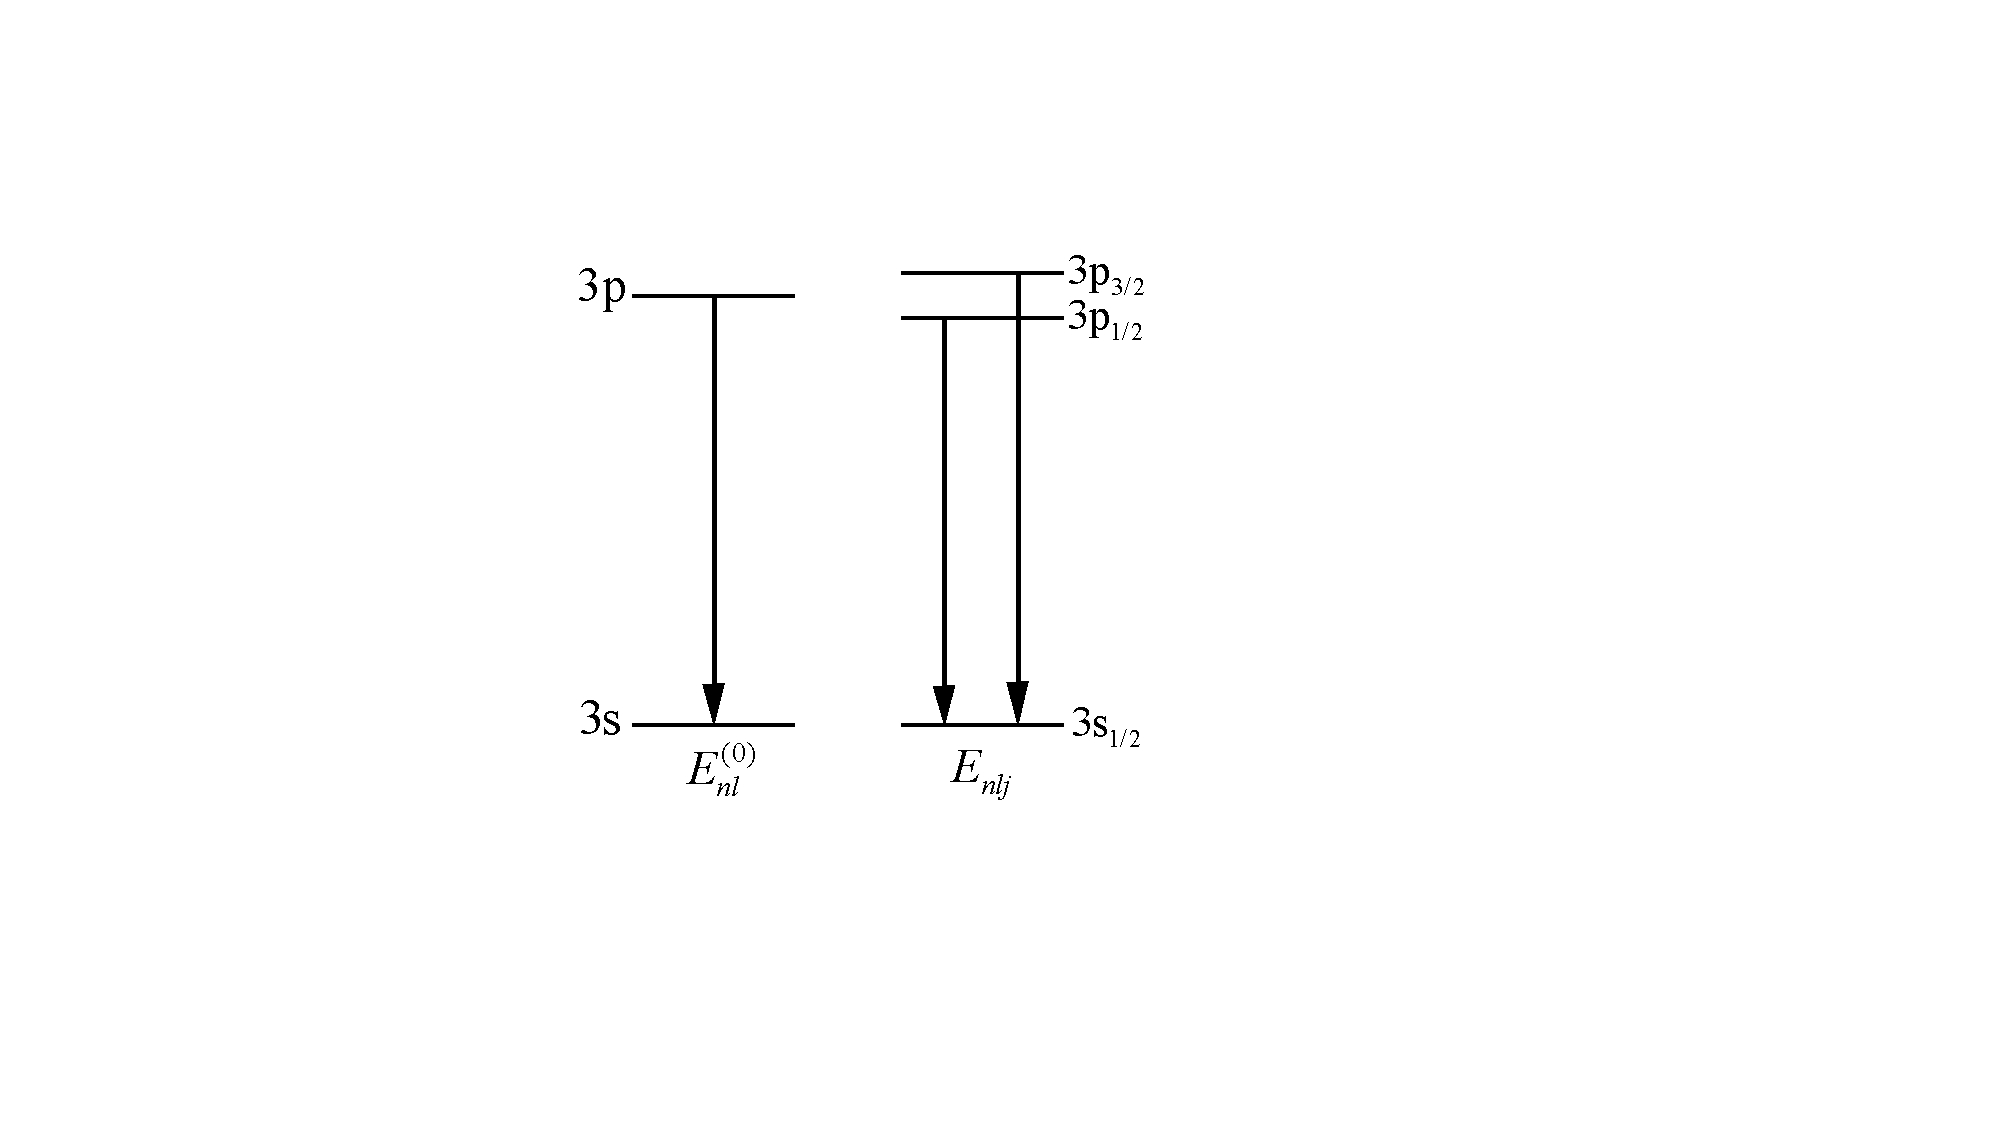
\includegraphics[width=3cm,clip]{QM file/figure/7-1}
	\caption{}\label{fig.7-1}
\end{wrapfigure}
由于自旋轨道耦合作用,能级$E_{nl}^{(0)}$分裂成两个能级,$j=l+\frac{1}{2}$者较高$(E_{nlj}^{(1)}>0)$,$j=l-\frac{1}{2}$者较低$(E_{nlj}^{(1)}<0)$,裂距
\eqllong
\begin{empheq}{align}\label{eq73.15}
	\Delta E&=E_{nl,l+\frac{1}{2}}^{(1)}-E_{nl,l-\frac{1}{2}}^{(1)}	\nonumber\\
	&=\bigg(l+\frac{1}{2}\bigg)\hbar^{2}\langle\xi(r)\rangle 
\end{empheq}\eqnormal
但s态例外,s态$\boldsymbol{S}\cdot\boldsymbol{L}\text{(本征值)}=0$,没有自旋轨道耦合能,能级不分裂.

能级分裂的示意图见图\ref{fig.7-1},图中画出了3p$(n=3,l=1)$能级的分裂情况与此相应,跃迁3p$\rightarrow$3s造成的光谱线也分裂成两条,这就是光谱线的精细结构.










% 粒子在电磁场中的运动
\starthis\section[粒子在电磁场中的运动]{粒子在电磁场中的运动} \label{sec:07.04} % 
% \makebox[5em][s]{} % 短题目拉间距

{\heiti 1. 自旋为零的粒子}

以$m$和$q$表示粒子的质量和电荷,而自旋为零.当粒子在电磁场中运动时,按照经典电动力学,哈密顿量为
\begin{empheq}{equation}\label{eq74.1}
	H=\frac{1}{2m}\bigg(\boldsymbol{p}-\frac{q}{c}\boldsymbol{A}\bigg)^{2}+q\phi
\end{empheq}
其中$\boldsymbol{p}$是粒子的正则动量,$\phi$和$\boldsymbol{A}$是电磁场的标势和矢势,它们与电场$\mathscr{E}$和磁场$B$的关系是
\begin{empheq}{equation}\label{eq74.2}
	\mathscr{E}=-\nabla\phi-\frac{1}{c}\frac{\partial\boldsymbol{A}}{\partial t},\quad \boldsymbol{B}=\nabla\times\boldsymbol{A}
\end{empheq}
由\eqref{eq74.1}式并利用正则方程
\begin{empheq}{equation}\label{eq74.3}
	\dot{x}_{i}=\frac{\partial H}{\partial p_{i}}\quad \dot{p}_{i}=-\frac{\partial H}{\partial x_{i}}
\end{empheq}
可以证明粒子的机械动量是
\begin{empheq}{equation}\label{eq74.4}
	m\boldsymbol{v}=m\frac{d}{dt}\boldsymbol{r}=\boldsymbol{p}-\frac{q}{c}\boldsymbol{A}
\end{empheq}
并可导出粒子的经典运动方程
\begin{empheq}{equation}\label{eq74.5}
	m\frac{d\boldsymbol{v}}{dt}=q\mathscr{E}+\frac{q}{c}\boldsymbol{v}\times\boldsymbol{B}
\end{empheq}
第一项为电场的作用力,第二项为磁场的作用力,即洛伦兹力.

推广到量子力学,只需将$\boldsymbol{p}$换成算符,即令
\eqshort
\begin{empheq}{equation}\label{eq74.6}
	\hat{\boldsymbol{p}}=-i\hbar\nabla
\end{empheq}\eqnormal
就得到哈密顿算符
\begin{empheq}{equation}\label{eq74.7}
	\hat{H}=\frac{1}{2m}\bigg(\hat{\boldsymbol{p}}-\frac{q}{c}\boldsymbol{A}\bigg)^{2}+q\phi
\end{empheq}
如定义速度算符
\begin{empheq}{equation}\label{eq74.8}
	\hat{\boldsymbol{v}}=\frac{d\hat{\boldsymbol{r}}}{dt}=\frac{1}{i\hbar}[\boldsymbol{r},\hat{H}]
\end{empheq}
容易求出
\begin{empheq}{equation}\label{eq74.9}
	\hat{\boldsymbol{v}}=\frac{1}{m}\bigg(\hat{\boldsymbol{p}}-\frac{q}{c}\boldsymbol{A}\bigg)
\end{empheq}
上式正是经典关系\eqref{eq74.4}式的量子力学推广.\eqref{eq74.7}式也可以写成
\begin{empheq}{equation}\label{eq74.10}
	\hat{H}=\frac{1}{2}m\hat{\boldsymbol{v}}^{2}+q\phi
\end{empheq}
\eqref{eq74.7}式中
\begin{empheq}{equation*}
	\bigg(\hat{\boldsymbol{p}}-\frac{q}{c}\boldsymbol{A}\bigg)^{2}=\hat{\boldsymbol{p}}^{2}+\frac{q^{2}}{c^{2}}\boldsymbol{A}^{2}-\frac{q}{c}(\hat{\boldsymbol{p}}\cdot\boldsymbol{A}+\boldsymbol{A}\cdot\hat{\boldsymbol{p}})
\end{empheq}
其中
\begin{empheq}{equation*}
	\hat{\boldsymbol{p}}\cdot\boldsymbol{A}+\boldsymbol{A}\cdot\hat{\boldsymbol{p}}=-i\hbar(\nabla\cdot\boldsymbol{A})+2\boldsymbol{A}\cdot\hat{\boldsymbol{p}}
\end{empheq}
即一般$\hat{\boldsymbol{p}}\cdot\boldsymbol{A}\neq\boldsymbol{A}\cdot\hat{\boldsymbol{p}}$.但如规定矢势$\boldsymbol{A}$满足横波条件$\nabla\cdot\boldsymbol{A}=0$,则$\boldsymbol{p}\cdot\boldsymbol{A}=\boldsymbol{A}\cdot\hat{\boldsymbol{p}}=-i\hbar\boldsymbol{A}\cdot\nabla$,这时$\hat{H}$可以化成
\eqlong
\begin{empheq}{align*}\label{eq74.7'}
	\hat{H}&=\frac{\hat{\boldsymbol{p}}^{2}}{2m}-\frac{q}{mc}\boldsymbol{A}\cdot\hat{\boldsymbol{p}}+\frac{q^{2}}{2mc^{2}}\boldsymbol{A}^{2}+q\phi	\\
	&=-\frac{\hbar^{2}}{2m}\nabla^{2}+i\frac{\hbar q}{mc}\boldsymbol{A}\cdot\nabla+\frac{q^{2}}{2mc^{2}}\boldsymbol{A}^{2}+q\phi	\tag{$7.4.7^{\prime}$}\eqnormal
\end{empheq}

薛定谔方程仍为
\eqshort
\begin{empheq}{equation}\label{eq74.11}
	i\hbar\frac{\partial}{\partial t}\varPsi=\hat{H}\varPsi 
\end{empheq}\eqnormal
写开来,就是
\eqllong
\begin{empheq}{equation*}\label{eq74.11'}
	i\hbar\frac{\partial\varPsi}{\partial t}=-\frac{\hbar^{2}}{2m}\nabla^{2}\varPsi+i\frac{\hbar q}{mc}\boldsymbol{A}\cdot\nabla\varPsi+\frac{q^{2}}{2mc^{2}}\boldsymbol{A}^{2}\varPsi+q\phi\varPsi	\tag{$7.4.11^{\prime}$}
\end{empheq}\eqnormal
下面导出连续性方程.上式的共轭方程为
\eqindent{2}
\begin{empheq}{equation*}\label{eq74.11''}
	i\hbar\frac{\partial\varPsi^{*}}{\partial t}=-\frac{\hbar^{2}}{2m}\nabla^{2}\varPsi^{*}+i\frac{\hbar q}{mc}\boldsymbol{A}\cdot\nabla\varPsi^{*}+\frac{q^{2}}{2mc^{2}}\boldsymbol{A}^{2}\varPsi^{*}+q\phi\varPsi^{*}	\tag{$7.4.11^{\prime\prime}$}
\end{empheq}\eqnormal
用$\varPsi^{*}$左乘\eqref{eq74.11'}式,$\varPsi$左乘\eqref{eq74.11''}式,相减,即得
\eqllong
\begin{empheq}{align*}
	i\hbar\frac{\partial}{\partial}(\varPsi^{*}\varPsi) =&-\frac{\hbar^{2}}{2m}(\varPsi^{*}\nabla^{2}\varPsi-\varPsi\nabla^{2}\varPsi^{*})	\\
	&+i\frac{\hbar q}{mc}\boldsymbol{A}\cdot(\varPsi^{*}\nabla+\varPsi\nabla\varPsi^{*})	\\
	=&-\frac{\hbar^{2}}{2m}\nabla\cdot(\varPsi^{*}\nabla\varPsi-\varPsi\nabla\varPsi^{*})+i\frac{\hbar q}{mc}\nabla\cdot(\boldsymbol{A}\varPsi^{*}\varPsi)
\end{empheq}\eqnormal
上式实质上就是连续性方程
\begin{empheq}{equation}\label{eq74.12}
	\frac{\partial\rho}{\partial t}+\nabla\cdot\boldsymbol{j}=0
\end{empheq}
其$\rho=\varPsi^{*}\varPsi$为概率密度,$\boldsymbol{j}$为概率流密度,
\begin{empheq}{equation}\label{eq74.13}
	\boldsymbol{j}=\frac{i\hbar}{2m}(\varPsi^{*}\nabla\varPsi-\varPsi\nabla\varPsi^{*})-\frac{q}{mc}\boldsymbol{A}\varPsi^{*}\varPsi
\end{empheq}
亦即
\begin{empheq}{align*}\label{eq74.13'}
	\boldsymbol{j}&=\frac{1}{2m}\varPsi^{*}\bigg(\hat{\boldsymbol{p}}-\frac{q}{c}\boldsymbol{A}\bigg)\varPsi+c.c.	\\
	&=\frac{1}{2}\varPsi^{*}\hat{\boldsymbol{v}}\varPsi+c.c.=\Re(\varPsi^{*}\hat{\boldsymbol{v}}\varPsi)
	\tag{$7.4.13^{\prime}$}
\end{empheq}
电荷密度及电流密度为
\begin{empheq}{align}
	&\rho_{n}=q\rho=q\varPsi^{*}\varPsi		\label{eq74.14}\\
	\boldsymbol{j}_{e}=q\boldsymbol{j}=\frac{q}{2}&\varPsi^{*}\hat{\boldsymbol{v}}\varPsi+c.c.=\Re(q\varPsi^{*}\hat{\boldsymbol{v}}\varPsi)		\label{eq74.15}
\end{empheq}
而在经典物理中$\boldsymbol{j}_{e}=\boldsymbol{v}\rho_{e}$.

{\heiti 2. 电子}

电子(电荷$q=-e$)具有自旋磁矩
\begin{empheq}{equation}\label{eq74.16}
	\boldsymbol{\mu}_{s}=-\frac{e}{m_{e}c}\boldsymbol{S}=-\frac{e\hbar}{2m_{n}c}\boldsymbol{\sigma}
\end{empheq}
当电子在电磁场中运动时,磁场$\boldsymbol{B}$对磁矩$\boldsymbol{\mu}_{s}$的作用势是
\begin{empheq}{equation}\label{eq74.17}
	-\boldsymbol{B}\cdot\boldsymbol{\mu}_{s}=\frac{e\hbar}{2m_{n}c}\boldsymbol{B}\cdot\boldsymbol{\sigma}
\end{empheq}
将\eqref{eq74.17}式和\eqref{eq74.7}式合起来,就是在电磁场中的电子哈密顿算符:
\begin{empheq}{equation}\label{eq74.18}
	\hat{H}=\frac{1}{2m_{e}}\bigg(\hat{\boldsymbol{p}}+\frac{e}{c}\boldsymbol{A}\bigg)^{2}-e\phi+\frac{e\hbar}{2m_{n}c}\boldsymbol{B}\cdot\boldsymbol{\sigma}
\end{empheq}
薛定谔方程形式上仍取\eqref{eq74.11}式的形式,但是波函数$\varPsi$($xyzS_{z}$表象)应表示成二分量的列矢量:
\begin{empheq}{equation}\label{eq74.19}
	\varPsi=\begin{bmatrix}
		\varPsi_{1}(xyz,t)	\\	\varPsi_{2}(xyz,t)
	\end{bmatrix}
\end{empheq}
薛定谔方程表现为
\begin{empheq}{equation}\label{eq74.20}
	i\hbar\frac{\partial}{\partial t}\begin{bmatrix}
		\varPsi_{1}	\\	\varPsi_{2}
	\end{bmatrix}=\hat{H}\begin{bmatrix}
		\varPsi_{1}	\\	\varPsi_{2}
\end{bmatrix}
\end{empheq}
习惯上称为泡利方程.仿照\eqref{eq74.11}式以下的步骤,不难导出连续性方程,从而得到概率密度$\rho$,概率流密度$\boldsymbol{j}$,电荷密度$\rho_{e}$,电流密度$\boldsymbol{j}_{e}$的公式.结果如下:
\begin{empheq}{equation}\label{eq74.21}
	\rho=\varPsi^{*}\varPsi=\varPsi_{1}^{*}\varPsi_{1}+\varPsi_{2}^{*}\varPsi_{2}	
\end{empheq}
\begin{empheq}{align}\label{eq74.22}
	\boldsymbol{j}&=\frac{1}{2m_{e}}\varPsi^{+}\bigg(\hat{\boldsymbol{p}}+\frac{e}{c}\boldsymbol{A}\bigg)\varPsi+c.c.=\Re(\varPsi^{*}\hat{\boldsymbol{v}}\varPsi)	\nonumber\\
	&=\Re(\varPsi_{1}^{*}\hat{\boldsymbol{v}}\varPsi_{1}+\varPsi_{2}^{*}\hat{\boldsymbol{v}}\varPsi_{2})
\end{empheq}
\begin{empheq}{equation}\label{eq74.23}
	\rho_{e}=-e\rho,\quad \boldsymbol{j}_{e}=-e\boldsymbol{j}
\end{empheq}
注意这些最均与自旋算符无关,因为它们反映电子的空间分布与流动情况,而自旋自由度与此无关.

{\heiti 3. 均匀磁场中的原子}

以单价原子为例,说明一下物质的磁性起源.原子的最外层电子(价电子)容易受外场的影响,原子的电磁性质在很大程度上取决于价电子.将原子置于均匀磁场中,以$\boldsymbol{B}$方向为$z$轴方向,则磁场为
\begin{empheq}{equation*}
	B_{x}=B_{y}=0,\quad B_{z}=B
\end{empheq}
矢势$\boldsymbol{A}$可以取为
\begin{empheq}{equation}\label{eq74.24}
	A_{x}=-\frac{B}{2}y,\quad A_{y}=\frac{B}{2}x,\quad A_{z}=0
\end{empheq}
并已满足横波条件$\nabla\cdot\boldsymbol{A}=0$,因此
\begin{empheq}{equation*}
	\hat{\boldsymbol{p}}\cdot\boldsymbol{A}=\boldsymbol{A}\cdot\hat{\boldsymbol{p}}=\frac{B}{2}(x\hat{p}_{y}-y\hat{p}_{x})=\frac{B}{2}\hat{L}_{z}
\end{empheq}
代入\eqref{eq74.18}式,[利用\eqref{eq74.7}式的展开\eqref{eq74.7'}式]得到
\eqllong
\begin{empheq}{equation}\label{eq74.25}
	\hat{H}=\frac{1}{2m_{e}}\hat{\boldsymbol{p}}^{2}+V(r)+\frac{eB}{2m_{e}c}(\hat{L}_{z}+2\hat{S}_{z})+\frac{e^{2}B^{2}}{8m_{e}c^{2}}(x^{2}+y^{2})
\end{empheq}
其中$V(r)$表示原子核与内层电子对于价电子的库仑作用势的总和,即\eqref{eq74.18}式中$(-e\phi)$项的等效表示.\eqref{eq74.25}式中前两项是原子中价电子本来的能量算符,后两项是磁作用能.由此可以求得原子的磁矩
\begin{empheq}{equation}\label{eq74.26}
	\hat{\mu_{z}}=-\frac{\partial\hat{H}}{\partial B}=-\frac{e}{2m_{e}c}(\hat{L}_{z}+2\hat{S}_{z})-\frac{e^{2}B}{4m_{e}c^{2}}(x^{2}+y^{2})
\end{empheq}\eqnormal
其中第一项是原子的固有磁矩(轨道磁矩及自旋磁矩).第二项与磁场$B$成正比,为诱导磁矩,它总是负的,属于逆磁性效应.按量级而言,第二项远小于第一项,因此只有固有磁矩为零的原子(如惰气原子及许多二价原子)逆磁性才能表现出来.

\eqref{eq74.26}式中,第一项量级与玻尔磁子相同,
\begin{empheq}{equation*}
	\mu_{B}=\frac{e\hbar}{2m_{e}c}=\num{5.8}\times 10^{-9}\si{eV/Gs}
\end{empheq}
第二项的量级约为
\eqlong
\begin{empheq}{align*}
	\frac{e^{2}B}{4m_{e}c^{2}}(x^{2}+y^{2})&\sim B\frac{e^{2}a_{0}^{2}}{4m_{e}c^{2}}\bigg(\frac{\hbar^{2}}{m_{e}e^{2}}\bigg)^{2}	\\
	&\sim\frac{B\mu_{B}^{2}}{m_{e}c^{2}}\bigg(\frac{\hbar c}{e^{2}}\bigg)^{2}\sim B\times10^{-18}\si{eV/Gs^{2}}
\end{empheq}
当$\boldsymbol{B}\sim10^{5}\si{Gs}$,第二项量级约为$10^{-13}\si{eV/Gs}$,仅为$\mu_{B}$的$10^{-4}$倍.

\example 求速度算符$\hat{\boldsymbol{v}}$各分量间的对易式.

\solution 以$[\hat{v}_{x},\hat{v}_{y}]$为例,按照\eqref{eq74.9}式,
\begin{empheq}{align}\label{eq74.27}
	[\hat{v}_{x},\hat{v}_{y}]&=\frac{1}{m^{2}}\bigg[\hat{p}_{x}-\frac{q}{c}A_{x},\quad \hat{p}_{y}-\frac{q}{c}A_{y}\bigg]	\nonumber\\
	&=-\frac{q}{m^{2}c}([\hat{p}_{x},A_{y}]+[A_{x},\hat{p}_{y}])	\nonumber\\	% $\hat{p}_{y}$?
	&=-\frac{q}{m^{2}c}(-i\hbar)\bigg(\frac{\partial A_{y}}{\partial x}-\frac{\partial A_{x}}{\partial y}\bigg)=i\frac{\hbar q}{m^{2}c}B_{z}
\end{empheq}\eqnormal
类似地有
\begin{empheq}{equation*}
	[\hat{v}_{y},\hat{v}_{z}]=i\frac{\hbar q}{m^{2}c}B_{x},\quad [\hat{v}_{z},\hat{v}_{x}]=i\frac{\hbar q}{m^{2}c}B_{y}
\end{empheq}
$\boldsymbol{B}=\nabla\times\boldsymbol{A}$写成矢量形式,就是
\begin{empheq}{equation*}\label{eq74.27'}
	\hat{\boldsymbol{v}}\times\hat{\boldsymbol{v}}=i\frac{\hbar q}{m^{2}c}\boldsymbol{B}
	\tag{$7.4.27^{\prime}$}
\end{empheq}
$\boldsymbol{B}=\nabla\times\boldsymbol{A}$
是磁场,进一步还可算出
\begin{empheq}{equation}\label{eq74.28}
	[\hat{\boldsymbol{v}},\hat{\boldsymbol{v}}^{2}]=i\frac{\hbar q}{m^{2}c}(\hat{\boldsymbol{v}}\times\boldsymbol{B}-\boldsymbol{B}\times\hat{\boldsymbol{v}})
\end{empheq}

% 塞曼效应
\section[塞曼效应]{塞曼效应} \label{sec:07.05} % 
% \makebox[5em][s]{} % 短题目拉间距

早在19世纪末就已经发现磁场能够影响原子光谱.1896年塞曼发现,如将光源放在磁场中,则每一条光谱线均分裂成一组相邻的线.这种现象称为塞曼效应.

显然, 谱线分裂的根源是能级分裂.以单价原子为例,其光谱产生于价电子的能级跃迁未加磁场前,价电子的能量算符可以写成(参看$\S$\ref{sec:07.03})
\begin{empheq}{equation}\label{eq75.1}
	H_{0}=\frac{\boldsymbol{p}^{2}}{2m_{e}}+V(r)+\xi(r)\boldsymbol{S}\cdot\boldsymbol{L}
\end{empheq}
最后一项是自旋轨道耦合能加上磁场后,价电子又获得一项磁作用势,以磁场方向为$z$轴,磁作用势为
\begin{empheq}{equation}\label{eq75.2}
	H^{\prime}=-\boldsymbol{B}\cdot(\boldsymbol{\mu_{L}}+\boldsymbol{\mu_{S}})=\frac{eB}{2m_{e}c}(L_{z}+2S_{z})
\end{empheq}
[参看\eqref{eq74.25}式,略去很小的逆磁性项($B^{2}$项).]价电子的总能量算符变成
\eqshort
\begin{empheq}{equation}\label{eq75.3}
	H=H_{0}+H^{\prime}
\end{empheq}\eqnormal
由$H^{\prime}$造成的能级分裂,视磁场的强弱而有所不同.

{\heiti 1. 强磁场,简单塞曼效应}

如磁场很强(至少要几十万高斯),以致\eqref{eq75.1}式中自旋轨道耦合能可以忽略不计,这时价电子的能量算符为
\begin{empheq}{equation}\label{eq75.4}
	H=\frac{\boldsymbol{p}^{2}}{2m_{e}}+V(r)+\frac{eB}{2m_{e}c}(L_{z}+2S_{z})
\end{empheq}
其中第三项为磁作用势.这时$H,H_{0},\boldsymbol{L}^{2},L_{z},S_{z}$是互相对易的守恒量.如以$E_{nl}^{(0)}$表示$H_{0}=(\hat{T}+V)$的本征值(未加磁场时的价电子能级),$\varPsi_{nlm}=R_{nl}(r)Y_{lm}(\theta\varphi)$表示$(H_{0},\boldsymbol{L}^{2},L_{z})$共同本征函数,则$(H,\boldsymbol{L}^{2},L_{z},S_{z})$的共同本征函数显然是
\begin{empheq}{equation}\label{eq75.5}
	\varPsi_{nlmm_{s}}=\varPsi_{nlm}\chi_{1/2},\quad \varPsi_{nlm}\chi_{-1/2}
\end{empheq}
前者$S_{z}=\frac{\hbar}{2}\bigg(m_{s}=\frac{1}{2}\bigg)$,后者$S_{z}=-\frac{\hbar}{2}\bigg(m_{s}=-\frac{1}{2}\bigg)$.能级可以记成$E=E_{nlmm_{s}}$,显然
\begin{empheq}{align}\label{eq75.6}
	E_{nlmm_{s}}&=E_{nl}^{(0)}+B\mu_{B}(m+2m_{s})	\nonumber\\
	&=E_{nl}^{(0)}+\begin{dcases}
		(m+1)B\mu_{B},\quad m_{s}=\frac{1}{2}	\\
		(m-1)B\mu_{B},\quad m_{s}=-\frac{1}{2}
	\end{dcases}
\end{empheq}
$\bigg(\mu_{B}$为玻尔磁子$\bigg)$上式表明,能级$E_{nl}^{(0)}$在磁场中分裂成一组等距离的能级,能级间距为$B\mu_{B}$.由能级跃迁产生的光谱线也有分裂现象,由于跃迁选择定则:
\begin{empheq}{equation}\label{eq75.7}
	\Delta l=\pm1,\quad \Delta m=0,\pm1,\quad \Delta m_{s}=0
\end{empheq}
的限制,每条谱线在磁场中分裂成三条等距离的谱线.能级和谱线的分裂如图\ref{fig.7-2}所示.

\begin{figure}[!h]
	\centering
	\small
	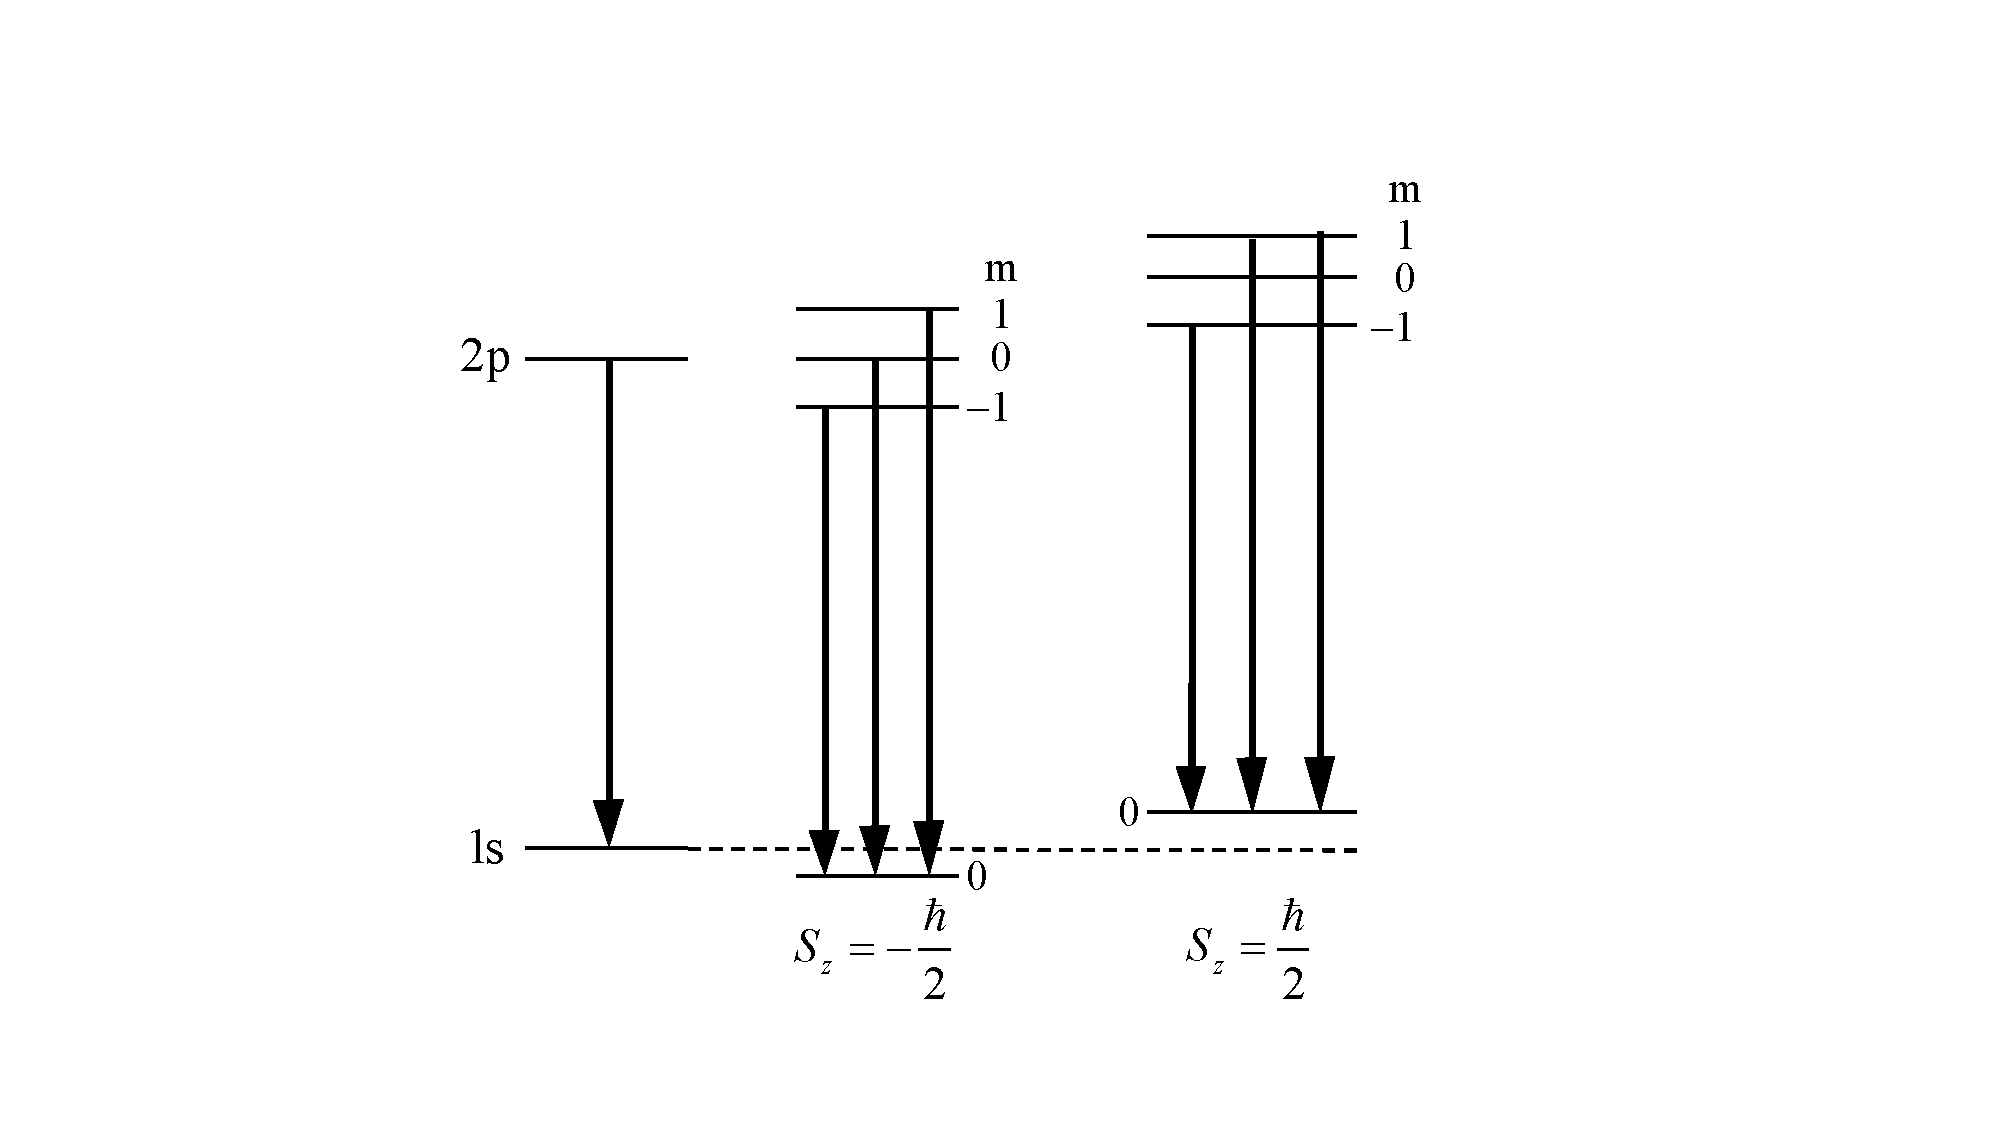
\includegraphics[width=5cm,clip]{QM file/figure/7-2}
	\caption{}\label{fig.7-2}
\end{figure}

图\ref{fig.7-2}画出了能级$E_{21}^{(0)}$,$E_{10}^{(0)}$在强磁场中的分裂示意图,以及符合选择定则的能级跃迁.由于跃迁前后自旋量子数$m_{s}$不变,图中两组跃迁产生的光谱相同,均包含三条谱线.相邻谱线的频率差为
\begin{empheq}{equation}\label{eq75.8}
	\Delta\omega=\frac{B\mu_{B}}{\hbar}=\frac{eB}{2m_{e}c}
\end{empheq}
刚好等于经典拉摩频率.这种现象,称为简单塞曼效应\footnote{
单价原子光谱在强磁场中的分裂现象,严格说应称为帕邢-巴克(Paschen-Back)效应.纯粹的简单塞曼效应只产生于价电子为偶数,总自旋角动量$S=0$的情况下,这时自旋轨道耦合能为0.磁作用势
\begin{empheq}{equation*}
	H^{\prime}=-\boldsymbol{B}\cdot\mu_{L}=\frac{eB}{2m_{e}c}L_{z}
\end{empheq}
($\boldsymbol{L}$为总轨道角动量)能级变化为$H^{\prime}=mB\mu_{B}(L_{z}=m\hbar)$,能级$E_{nl}^{(0)}$分裂成$(2L+1)$条等距离能级,间距$\Delta E=B\mu_{B}$.由于跃迁选择定则\eqref{eq75.7}式的制约,光谱线仍分裂为三条等距离的谱线,$\Delta\omega$仍由\eqref{eq75.8}式表示.这种效应只需要弱磁场就能产生,而且可以给以经典电动力学解释,所以曾称为正常塞曼效应.其实下面要讲的复杂塞曼效应才是塞曼效应的一般表现形式,由于它无法用经典物理理论来解释,曾被称为“反常”的.}由于$\Delta\omega$与$\hbar$无关,历史上曾根据经典电动力学的拉摩进动模型给出了很好的定量解释.

{\heiti 2. 弱磁场,复杂塞曼效应}

在弱磁场中,单价原子受到的磁作用势小于自旋轨道耦合能,应将\eqref{eq75.3}式中$H^{\prime}$作为微扰.取$(H_{0},\boldsymbol{L}^{2},\boldsymbol{J}^{2},J_{z})$共同本征函数作为零级近似波函数,记为
\begin{empheq}{equation}\label{eq75.9}
	\Psi_{nljm_{j}}^{(0)}=R_{nl}(r)\varPsi_{ljm_{j}}(\theta,\varphi,S_{z})
\end{empheq}
其中$\varPsi_{ljm_{j}}$表示$(\boldsymbol{L}^{2},\boldsymbol{J}^{2},J_{z})$共同本征函数(见$\S$\ref{sec:07.02}).$H_{0}$由\eqref{eq75.1}式表示,其中包含了自旋轨道耦合能.$H_{0}$的本征值即未加磁场时的价电子能级,和量子数$nlj$有关,但和$m_{j}$无关,(见$\S$\ref{sec:07.03})可以记为$E_{nlj}^{(0)}$,能级简并度$(2j+1)$.给定$n,l$后,$j=l\pm\frac{1}{2}$对应于两个能级,就是能级的精细结构(见$\S$\ref{sec:07.03}).

按照简并态微扰论计算磁作用势$H^{\prime}$造成的能级变化(一级修正).由于$H^{\prime}$与$J_{z}$对易,因此$H^{\prime}$的非对角矩阵元全部等于0,能级的一级修正等于$H^{\prime}$对\eqref{eq75.9}式的平均值,即
\eqlong
\begin{empheq}{align}\label{eq75.10}
	E_{nljm_{j}}^{(1)} &=\int\Psi_{nljm_{j}}^{(0)+}\hat{H}\Psi_{nljm_{j}}^{(0)}d\tau	\nonumber\\
	&=\frac{eB}{2m_{e}c}(\overline{J_{z}}+\overline{S_{z}})=\frac{eB}{2m_{e}c}\bigg(m_{j}\hbar+\frac{\hbar}{2}\overline{\sigma_{z}}\bigg)
\end{empheq}\eqnormal
其中$\overline{\sigma_{z}}$已在\eqref{eq72.23}式、\eqref{eq72.24}式算出,为
\begin{empheq}{align}\label{eq75.11}
	\overline{\sigma_{z}}=
	\begin{dcases}
		\quad\frac{m_{j}}{j},\qquad j=l+\frac{1}{2}	\\
		-\frac{m_{j}}{j+1},\quad j=l-\frac{1}{2}
	\end{dcases}
\end{empheq}
代入\eqref{eq75.10}式, 即得
\begin{empheq}{equation}\label{eq75.12}
	E_{nljm_{j}}^{(1)}=B\mu_{B}m_{j}g
\end{empheq}
其中$g$为朗德$g$因子,即
\eqlong
\begin{empheq}{align}\label{eq75.13}
	g &=1+\frac{\langle\sigma_{z}\rangle}{2m_{j}}=1+\frac{\langle S_{z}\rangle}{\langle J_{z}\rangle}	\\
	&=\begin{dcases}
		1+\frac{1}{2j},\qquad\quad	j=l+\frac{1}{2}	\\
		1-\frac{1}{2j+2},\quad j=l-\frac{1}{2}	
	\end{dcases}	\nonumber \tag{$7.5.13^{\prime}$}
\end{empheq}\eqnormal
这样, 由\eqref{eq75.12}式、\eqref{eq75.13}式可知,能级$E_{nlj}^{(0)}$在弱磁场中分裂成$(2j+1)$个等距离能级,相应于$m_{j}$的$(2j+1)$种取值
\begin{empheq}{equation}\label{eq75.14}
	m_{j}=j,j-1,\cdots,(-j)
\end{empheq}
能级间距为$B\mu_{B}g$.(在简单塞曼效应中,能级分裂间距为$B\mu_{B}$)因此,对光谱进行实验分析浏定,可以推断出能级的$g$和$j$值(由此也就知道$l$值),这样就获得了有关原子结构的重要信息.

能级跃迁的选择定则是
\begin{empheq}{equation}\label{eq75.15}
	\Delta l=\pm1,\quad \Delta j=0,\pm1,\quad \Delta m_{j}=0,\pm1
\end{empheq}
图\ref{fig.7-3}画出了钠(\ce{Na})的$D_{1}$和$D_{2}$线的分裂示意图.能级和谱线的分裂均比简单塞曼效应复杂,故称复杂塞曼效应.发现这现象的当时,无法对此作出理论解释,故又称反常塞曼效应.直到1925年乌仑贝克(Uhlenbeck)与古兹米特(Goudsmit)提出电子自旋假设,这个“反常”现象才得到解释.

\begin{figure}[!h]
	\centering
	\small
	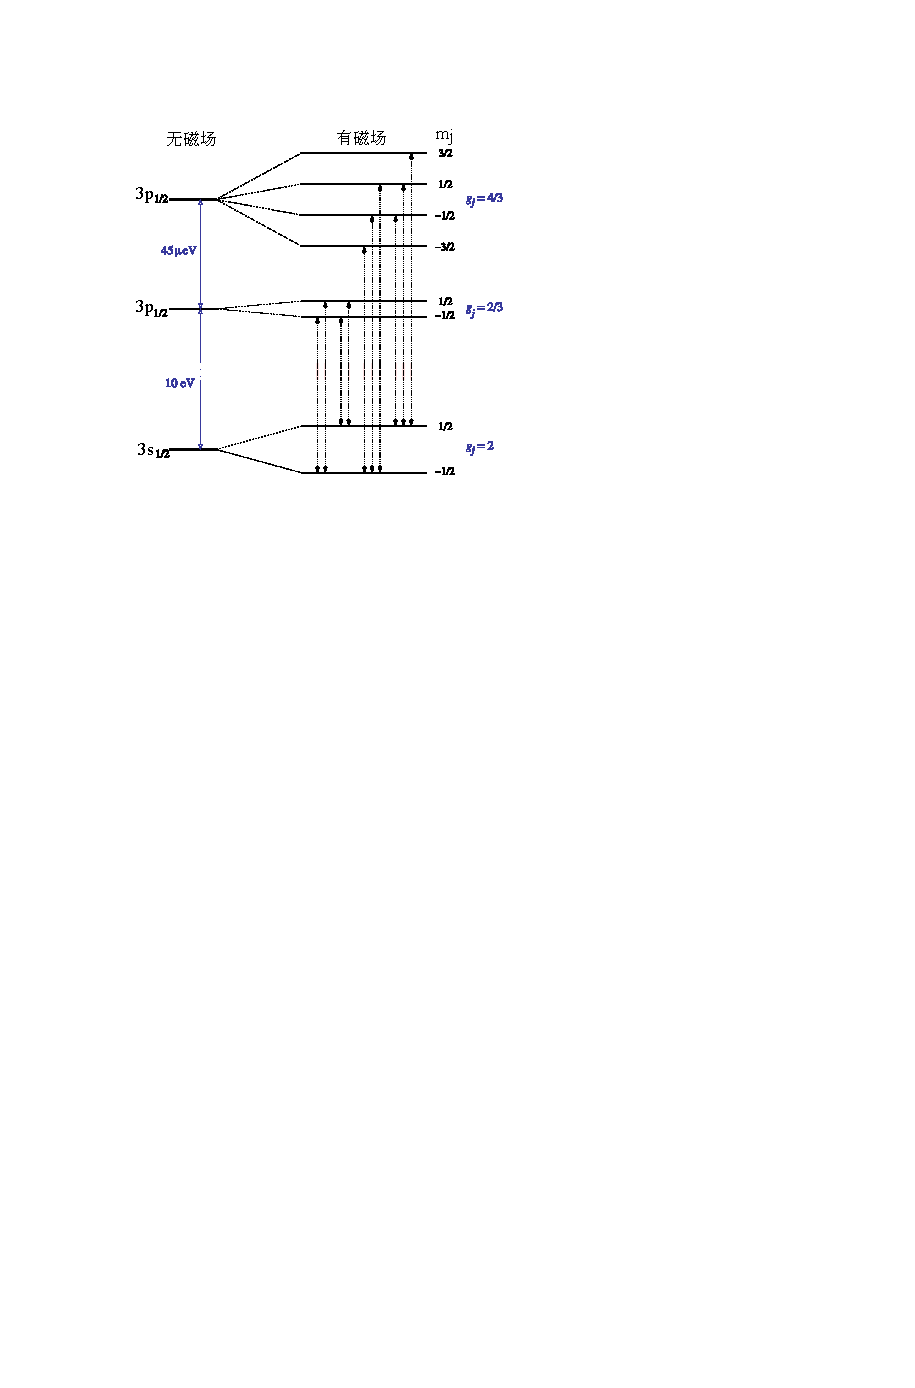
\includegraphics[width=5cm,clip]{QM file/figure/7-3}
	\caption{}\label{fig.7-3}
\end{figure}


\example 证明朗德$g$因子也可以表示成
\eqlong
\begin{empheq}{equation}\label{eq75.16}
	g=1+\frac{j(j+1)+s(s+1)-l(l+1)}{2j(j+1)}\quad \bigg(s=\frac{1}{2}\bigg)
\end{empheq}\eqnormal

\solution 由\eqref{eq72.27}式,可得(以下各式中,$\boldsymbol{\sigma}\cdot\boldsymbol{L}$均指其本征值.$\hbar$均略去不写)
\eqshort
\begin{empheq}{equation}\label{eq75.17}
	\overline{S_{z}}=\frac{m_{j}}{1+2\boldsymbol{\sigma}\cdot\boldsymbol{L}}
\end{empheq}\eqnormal
而\eqref{eq72.5}式取本征值,有
\begin{empheq}{equation}\label{eq75.18}
	j(j+1)=l(l+1)+\frac{3}{4}+\boldsymbol{\sigma}\cdot\boldsymbol{L}
\end{empheq}
利用\eqref{eq72.11}式消去$l(l+1)$,成为
\begin{empheq}{equation}\label{eq75.19}
	\begin{aligned}
		j(j+1)&=(\boldsymbol{\sigma}\cdot\boldsymbol{L})^{2}+2\boldsymbol{\sigma}\cdot\boldsymbol{L}+\frac{3}{4}	\\
		&=\bigg(\boldsymbol{\sigma}\cdot\boldsymbol{L}+\frac{1}{2}\bigg)\bigg(\boldsymbol{\sigma}\cdot\boldsymbol{L}+\frac{3}{2}\bigg)
	\end{aligned}
\end{empheq}
利用此式,可将\eqref{eq75.17}式变成
\begin{empheq}{align}\label{eq75.20}
	\frac{\overline{S_{z}}}{m_{j}} &=\frac{\boldsymbol{\sigma}\cdot\boldsymbol{L}+\frac{3}{2}}{2j(j+1)},\text{再\eqref{eq75.18}利用式,}	\nonumber\\
	&=\frac{j(j+1)+\frac{3}{4}-l(l+1)}{2j(j+1)}
\end{empheq}
再代入\eqref{eq75.13}式,即得
\eqlong
\begin{empheq}{equation*}
	g=1+\frac{\overline{S_{z}}}{m_{j}\hbar}=1+\frac{j(j+1)+\frac{3}{4}-l(l+1)}{2j(j+1)}
\end{empheq}\eqnormal
此即\eqref{eq75.16}式.

% 磁共振
\starthis\section[磁共振]{磁共振} \label{sec:07.06} % 
% \makebox[5em][s]{} % 短题目拉间距

磁共振的基本原理是利用粒子的磁矩在交变磁场中作周期性变化的规律,对磁矩或磁场作精密测量.

以自旋为$\frac{\hbar}{2}$的粒子为例,自旋磁矩算符可以表示成
\eqshort
\begin{empheq}{equation}\label{eq76.1}
	\boldsymbol{\mu}=\mu_{0}\boldsymbol{\sigma}
\end{empheq}\eqnormal
$\boldsymbol{\sigma}$为泡利算符,$\mu_{0}$由粒子性质决定,对于电子,$\mu_{0}=-\frac{e\hbar}{2m_{e}c}$.将粒子置于恒定磁场$B_{0}$中,(以磁场方向为$z$轴方向)则磁作用势(略去与自旋无关的项)为
\begin{empheq}{equation}\label{eq76.2}
	\hat{H}_{0}=-B_{0}\cdot\boldsymbol{\mu}=-B_{0}\mu_{0}\sigma_{z}
\end{empheq}
这时$\sigma_{z}$是守恒量(和$H_{0}$对易),它的本征态$\chi_{1/2}$及$\chi_{-1/2}$也是$H_{0}$的本征态,相应的能级为
\begin{empheq}{equation}\label{eq76.3}
	E_{\pm}=\mp B_{0}\mu_{0}=\mp\hbar\omega,\quad \omega=\frac{B_{0}\mu_{0}}{\hbar}
\end{empheq}
现在再加上一个和$B_{0}$垂直的交变磁场$B_{1}(t)$,
\begin{empheq}{equation}\label{eq76.4}
	B_{1x}=B_{1}\cos\nu t,\quad B_{1y}=-B_{1}\sin\nu t,\quad B_{1z}=0
\end{empheq}
磁作用势变成
\begin{empheq}{align}\label{eq76.5}
	\hat{H} &=-(B_{0}+B_{1})\cdot\boldsymbol{\mu}	\nonumber\\
	&=-B_{0}\mu_{0}\sigma_{z}+B_{1}\mu_{0}(\sigma_{y}\sin\nu t-\sigma_{x}\cos\nu t)
\end{empheq}
如将$H$在$\sigma_{z}$表象中写成矩阵形式,就是
\begin{empheq}{equation*}\label{eq76.5'}
	\hat{H}=-\mu_{0}\begin{bmatrix}
		B_{0} & B_{1}e^{i\nu t}	\\
		B_{1}e^{-i\nu t} & -B_{0} \\
	\end{bmatrix}
\end{empheq}

设在$t=0$时粒子自旋指向$z$方向,即初始自旋波函数为
\eqshort
\begin{empheq}{equation}\label{eq76.6}
	\chi(t=0)=\chi_{1/2}=\begin{bmatrix}
		1 \\  0
	\end{bmatrix}
\end{empheq}
在$t>0$时,由于$B_{1}$场的存在,$\sigma_{z}$不再是守恒量,自旋波函数将按照薛定谔方程
\begin{empheq}{equation}\label{eq76.7}
	i\hbar\frac{d}{dt}\chi(t)=\hat{H}\chi(t)
\end{empheq}\eqnormal
随$t$变化,$\chi(t)$可以表示成
\begin{empheq}{equation}\label{eq76.8}
	\chi(t)=C_{1}(t)\chi_{1/2}+C_{2}(t)\chi_{-1/2}=\begin{bmatrix}
		C_{1}(t)	\\	C_{2}(t)
	\end{bmatrix}
\end{empheq}
将\eqref{eq76.5'}及\eqref{eq76.8}式代入\eqref{eq76.7}式,得到$C_{1},C_{2}$的联立方程
\begin{empheq}{equation}\label{eq76.9}
	{}\begin{dcases}
		i\hbar\dot{C_{1}}=-\mu_{0}B_{0}C_{1}-\mu_{0}B_{1}e^{i\nu t}C_{2}	\\
		i\hbar\dot{C_{2}}=\mu_{0}B_{0}C_{2}-\mu_{0}B_{1}e^{-i\nu t}C_{1}
	\end{dcases}
\end{empheq}
令
\begin{empheq}{equation}\label{eq76.10}
	C_{1}=a(t)e^{i\nu t/2},\quad C_{2}=b(t)e^{-i\nu t/2}
\end{empheq}
可将\eqref{eq76.9}式简化成
\eqlong
\begin{empheq}{equation}\label{eq76.11}
	{}\begin{dcases}
		\dot{a}=i\bigg(\omega-\frac{\nu}{2}\bigg)a+i\gamma\omega b
		\dot{b}=-i\bigg(\omega-\frac{\nu}{2}\bigg)b+i\gamma\omega a
	\end{dcases}\eqnormal
\end{empheq}
其中
\eqshort
\begin{empheq}{equation}\label{eq76.12}
	\omega=\frac{\mu_{0}B_{0}}{\hbar},\quad \gamma=\frac{B_{1}}{B_{0}}
\end{empheq}\eqnormal
实验测量是在“共振条件”$\nu=2\omega$情况下进行,这时\eqref{eq76.11}式成为
\begin{empheq}{equation}\label{eq76.13}
	{}\begin{dcases}
		\dot{a}=i\gamma\omega b
		\dot{b}=i\gamma\omega a
	\end{dcases}\quad (\nu=2\omega)
\end{empheq}
解为
\begin{empheq}{equation*}
	a(t)\pm b(t)=[a(0)\pm b(0)]e^{\pm i\gamma\omega t}
\end{empheq}
根据初始条件\eqref{eq76.6}式,$a(0)=1,b(0)=0$,因此
\eqshort
\begin{empheq}{equation*}
	a(t)\pm b(t)=e^{\pm i\gamma\omega t}
\end{empheq}\eqnormal
解出
\begin{empheq}{equation}\label{eq76.14}
	a(t)=\cos\gamma\omega t,\quad b(t)=i\sin\gamma\omega t
\end{empheq}
代入\eqref{eq76.8}式、\eqref{eq76.10}式,就得到自旋波函数
\begin{empheq}{align}\label{eq76.15}
	\chi(t) &=\cos\gamma\omega e^{i\omega t}\chi_{1/2}+i\sin\gamma\omega t e^{-i\omega t}\chi_{-1/2}	\nonumber\\
	&=\begin{bmatrix}
		\cos\gamma\omega te^{i\omega t}	\\
		i\sin\gamma\omega te^{-i\omega t}
	\end{bmatrix}
\end{empheq}
以$t=0$时粒子的初始自旋方向(正$z$轴方向,$\sigma_{z}=1$)为标准,在时刻$t$自旋方向反转$(\sigma_{z}=-1)$的概率为
\eqshort
\begin{empheq}{equation}\label{eq76.16}
	|C_{2}|^{2}=\sin^{2}\gamma\omega t
\end{empheq}\eqnormal
当$t=\frac{\pi}{2\gamma\omega}=\frac{\pi\hbar}{2\mu_{0}B_{1}}$,粒子自旋方向刚好完全反转.($C_{1}=0$,\eqref{eq76.15}式中只有$\chi_{-1/2}$几项)

在非共振条件下,即$\nu\neq\omega$时,\eqref{eq76.11}式仍存在振动解,令
\begin{empheq}{equation}\label{eq76.17}
	{}\begin{dcases}
		a(t)=a_{1}e^{i\Omega t}+a_{2}e^{-i\Omega t}	\\
		b(t)=b_{1}e^{i\Omega t}+b_{2}e^{-i\Omega t}
	\end{dcases}
\end{empheq}
代入\eqref{eq76.11}式,容易得到存在非平庸解($a_{1},a_{2},b_{1},b_{2}$不全为0)的条件为
\begin{empheq}{equation*}
	\begin{vmatrix}
		\omega+\bigg(\omega-\frac{\nu}{2}\bigg)	& \gamma\omega \\
		\gamma\omega & \Omega-\bigg(\omega-\frac{\nu}{2}\bigg)	
	\end{vmatrix}=0
\end{empheq}
解出
\begin{empheq}{equation}\label{eq76.18}
	\Omega=\bigg[\bigg(\omega-\frac{\nu}{2}\bigg)^{2}+\gamma^{2}\omega^{2}\bigg]^{1/2}
\end{empheq}
考虑到初始条件\eqref{eq76.6}式,即$a(0)=1,b(0)=0$,\eqref{eq76.17}式可以写成
\begin{empheq}{equation*}\label{eq76.17'}
	{}\begin{dcases}
		a(t)=\cos\Omega t+a_{3}\sin\Omega t	\\
		b(t)=b_{3}\sin\Omega t
	\end{dcases}
\end{empheq}
代入\eqref{eq76.11}式,并利用\eqref{eq76.18}式,求出
\begin{empheq}{equation*}
	a_{3}=i\frac{\omega-\frac{\nu}{2}}{\Omega},\quad b_{3}=i\frac{\gamma\omega}{\Omega}
\end{empheq}
\begin{empheq}{equation}\label{eq76.19}
	{}\begin{dcases}
		a(t)=\cos\Omega t+i\frac{\omega-\frac{\nu}{2}}{\Omega}\sin\Omega t	\\
		b(t)=i\frac{\gamma\omega}{\Omega}\sin\Omega t
	\end{dcases}
\end{empheq}
注意,在共振条件$(\nu=2\omega)$下,$\Omega=\gamma\omega$,\eqref{eq76.19}式变成\eqref{eq76.14}式.由\eqref{eq76.8}式、\eqref{eq76.10}式、\eqref{eq76.19}式可知,非共振条件下,时刻$t$自旋方向反转概率
\begin{empheq}{equation}\label{eq76.20}
	|b(t)|^{2}=\bigg(\frac{\gamma\omega}{\Omega}\bigg)^{2}\sin^{2}\Omega t
\end{empheq}
显然
\begin{empheq}{equation}\label{eq76.21}
	|b(t)|_{\text{极大}}^{2}=\bigg(\frac{\gamma\omega}{\Omega}\bigg)^{2}<1
\end{empheq}
而在共振条件下$(\nu=2\omega)$自旋方向反转概率最大可以达到1.

粒子自旋方向的反转,相当于在磁能级$E_{+},E_{-}$间的跃迁,与此相应,粒子从电磁波(交变磁场)中吸收能量
\begin{empheq}{equation}\label{eq76.22}
	\hbar\nu=2\hbar\omega=E_{-}-E_{+}=2B_{0}\mu_{0}
\end{empheq}
在磁共振实验中,交变磁场的频率$\nu$可以调整,当达到共振条件$(\nu=2\omega)$时,出现交变场功率的吸收峰.如$B_{0}$已经精确给定,利用\eqref{eq76.22}式就可测出粒子磁矩$\mu_{0}$.反之,如$\mu_{0}$已知,则可测定$B_{0}$.由于$2\omega$是在射频至微波频段,测量可以达到很高的精度.

对于化合物或凝聚态物质,由于存在自旋轨道耦合作用以及原子间互作用,磁矩结构及磁能级较为复杂,利用磁共振技术可以获得物质结构单元的磁矩信息,有助于了解材料的结构.


% 两个角动量的耦合
\section[两个角动量的耦合]{两个角动量的耦合} \label{sec:07.07} % 
% \makebox[5em][s]{} % 短题目拉间距

电子的自旋角动量与轨道角动量相加成总角动盘($\S$\ref{sec:07.02})是角动量耦合的一个实例.本节讨论一般的角动量耦合问题.

设$\boldsymbol{J}_{1}$和$\boldsymbol{J}_{2}$是属于不同自由度的角动量算符,它们互相对易:
\begin{empheq}{equation}\label{eq77.1}
	[J_{1\alpha},J_{2\beta}]=0,\quad \alpha,\beta = x,y,z
\end{empheq}
而又各自满足角动量对易式:
\begin{empheq}{equation}\label{eq77.2}
	\boldsymbol{J}_{1}\times\boldsymbol{J}_{1}=i\hbar\boldsymbol{J}_{1},\quad \boldsymbol{J}_{2}\times\boldsymbol{J}_{2}=i\hbar\boldsymbol{J}_{2}
\end{empheq}
因此必然有
\begin{empheq}{equation}\label{eq77.3}
	[\boldsymbol{J}_{1}^{2},\boldsymbol{J}_{1}]=0,\quad [\boldsymbol{J}_{2}^{2},\boldsymbol{J}_{2}]=0
\end{empheq}
以$\boldsymbol{J}$表示$\boldsymbol{J}_{1},\boldsymbol{J}_{2}$之和,即
\begin{empheq}{equation}\label{eq77.4}
	\boldsymbol{J}=\boldsymbol{J}_{1}+\boldsymbol{J}_{2}
\end{empheq}
则
\begin{empheq}{equation}\label{eq77.5}
	\boldsymbol{J}^{2}=\boldsymbol{J}_{1}^{2}+\boldsymbol{J}_{2}^{2}+2\boldsymbol{J}_{1}\cdot\boldsymbol{J}_{2}
\end{empheq}
由\eqref{eq77.1}式,易知
\begin{empheq}{align}
	\boldsymbol{J}_{1}\cdot\boldsymbol{J}_{2}&=\boldsymbol{J}_{2}\cdot\boldsymbol{J}_{1}	\label{eq77.6}\\
	\boldsymbol{J}_{1}\times\boldsymbol{J}_{2}&=-\boldsymbol{J}_{2}\times\boldsymbol{J}_{1}	\label{eq77.7}
\end{empheq}
因此
\eqlong
\begin{empheq}{align}\label{eq77.8}
	\boldsymbol{J}\times\boldsymbol{J}&=\boldsymbol{J}_{1}\times\boldsymbol{J}_{1}+\boldsymbol{J}_{2}\times\boldsymbol{J}_{2}+\boldsymbol{J}_{1}\times\boldsymbol{J}_{2}+\boldsymbol{J}_{2}\times\boldsymbol{J}_{1}	\nonumber\\
	&=i\hbar\boldsymbol{J}_{1}+i\hbar\boldsymbol{J}_{2}=i\hbar\boldsymbol{J}
\end{empheq}\eqnormal
因此$\boldsymbol{J}$也是角动量容易证明
\eqshort
\begin{empheq}{equation}\label{eq77.9}
	[\boldsymbol{J}^{2},\boldsymbol{J}]=0
\end{empheq}\eqnormal
利用\eqref{eq77.3}式容易证明
\begin{empheq}{equation}\label{eq77.10}
	[\boldsymbol{J}_{1}^{2},\boldsymbol{J}]=0,\quad [\boldsymbol{J}_{2}^{2},\boldsymbol{J}]=0
\end{empheq}
因此,$\boldsymbol{J}_{1}^{2},\boldsymbol{J}_{2}^{2},\boldsymbol{J}^{2},J_{z}$互相对易,可以选作力学量完全集.
\pskip

$\S$\ref{sec:04.07}中关于角动量的一般理论对于这里的$\boldsymbol{J}_{1},\boldsymbol{J}_{2}$和$\boldsymbol{J}$均可适用.以$\varPsi_{j_{1}m_{1}}$或$|j_{1}m_{1}\rangle$表示$(\boldsymbol{J}_{1}^{2},J_{1z})$共同本征态,即设
\eqlong
\begin{empheq}{equation}\label{eq77.11}
	\begin{aligned}
		\boldsymbol{J}_{1}^{2}\varPsi_{j_{1}m_{1}} &=j_{1}(j+1)\hbar^{2}\varPsi_{j_{1}m_{1}}	\\
		J_{1z}\varPsi_{j_{1}m_{1}} &=m_{1}\hbar\varPsi_{j_{1}m_{1}},\quad m_{1}=j_{1},j_{1}-1,\cdots(-j_{1})
	\end{aligned}
\end{empheq}
按照$\S$\ref{sec:04.07},升降算符的作用结果是
\eqllong
\begin{empheq}{equation}\label{eq77.12}
	(J_{1x}\pm iJ_{1y})\varPsi_{j_{1}m_{1}}=\hbar\sqrt{(j_{1}\pm m_{1}+1)(j_{1}\mp m_{1})}\varPsi_{j_{1}m_{1}\pm 1}
\end{empheq}
类似地,以$\varPsi_{j_{2}m_{2}}$或$|j_{2}m_{2}\rangle$表示$(\boldsymbol{J}_{2}^{2},J_{2z})$共同本征态,也有类似于\eqref{eq77.11}式、\eqref{eq77.12}式的公式,不再一一写出.
\pskip

$(\boldsymbol{J}_{1}^{2},\boldsymbol{J}_{2}^{2},\boldsymbol{J}^{2},J_{z})$共同本征态记为$\varPsi_{j_{1}j_{2}jM}$或$|j_{1}j_{2}jM\rangle$,相应于本征值
\begin{empheq}{equation}\label{eq77.13}
	\begin{aligned}
		&\boldsymbol{J}_{1}^{2}=j_{1}(j_{1}+1)\hbar^{2},\quad &\boldsymbol{J}_{2}^{2}=j_{2}(j_{2}+1)\hbar^{2}			\\
		&\boldsymbol{J}^{2}=j(j+1)\hbar^{2},\quad 
		&J_{z}=M\hbar,M=j,j-1,\cdots,(-j)
	\end{aligned}
\end{empheq}\eqlong
首先要解决的问题是,当$j_{1}$与$j_{2}$给定后,$j$有哪些可能取值.其次的问题是,$\varPsi_{j_{1}j_{2}jM}$态和$\varPsi_{j_{1}m_{1}}$及$\varPsi_{j_{2}m_{2}}$态是什么关系.按照$\S$\ref{sec:07.02}的经验,$\varPsi_{j_{1}j_{2}jM}$显然可以表示成
\begin{empheq}{equation}\label{eq77.14}
	\varPsi_{j_{1}j_{2}jM}=\sum_{m_{1}}\sum_{m_{2}}C(j,M,m_{1},m_{2})\varPsi_{j_{1}m_{1}}\varPsi_{j_{2}m_{2}}
\end{empheq}\eqnormal
由于$J_{z}=J_{1z}+J_{2z}$,显然有
\begin{empheq}{equation}\label{eq77.15}
	J_{z}\varPsi_{j_{1}m_{1}}\varPsi_{j_{2}m_{2}}=(m_{1}+m_{2})\hbar\varPsi_{j_{1}m_{1}}\varPsi_{j_{2}m_{2}}
\end{empheq}
因此\eqref{eq77.14}式中只包含$m_{1}+m_{2}=M$的项.给定$j_{1},j_{2}$后,$m_{1}$共有$(2j_{1}+1)$种取值(依次相差1),$m_{2}$共有$(2j_{2}+1)$种取值(依次相差1),故\eqref{eq77.14}式右端最多有$(2j_{1}+1)(2j_{2}+1)$种独立项,最多能组成同样数目的独立的$\varPsi_{j_{1}j_{2}jM}$.其中对于某个$j$值,相应的$M$值有$(2j+1)$种,即
\begin{empheq}{equation*}
	M=j,j-1,\cdots,(-j)
\end{empheq}
由于$M$值只能依次相差1,所以$j$也只能依次相差1.$M$的最大值显然是$(j_{1}+j_{2})$,这也就是$j$的最大值.因此,$j$的可能取值为
\begin{empheq}{equation*}
	j=j_{1}+j_{2},j_{1}+j_{2}-1,\cdots,j_{min}
\end{empheq}
由此可知,独立的$\varPsi_{j_{1}j_{2}jM}$总数为
\begin{empheq}{equation*}
	N=\sum_{j}(2j+1)=(j_{1}+j_{2}+j_{min}+1)(j_{1}+j_{2}-j_{min}+1)
\end{empheq}
上式应等于$(2j_{1}+1)(2j_{2}+1)$,为此必须$j_{min}=|j_{1}-j_{2}|$.因此,$j$的取值为
\begin{empheq}{equation}\label{eq77.16}
	\boxed{j=j_{1}+j_{2},j_{1}+j_{2}-1,\cdots,|j_{1}-j_{2}|}
\end{empheq}
量子数$j_{1},j_{2}$,$j$之间的这种关系常被形象地称为三角形条件,记为$\Delta(j_{1}j_{2}j)$,或用图\ref{fig.7-4}表示,但必须记住,$j$是量子化的,所以图中$j_{1},j_{2}$的夹角也必须是量子化的,以保证\eqref{eq77.16}式成立.

\begin{wrapfigure}[8]{r}{7em}
	\centering
	\small
	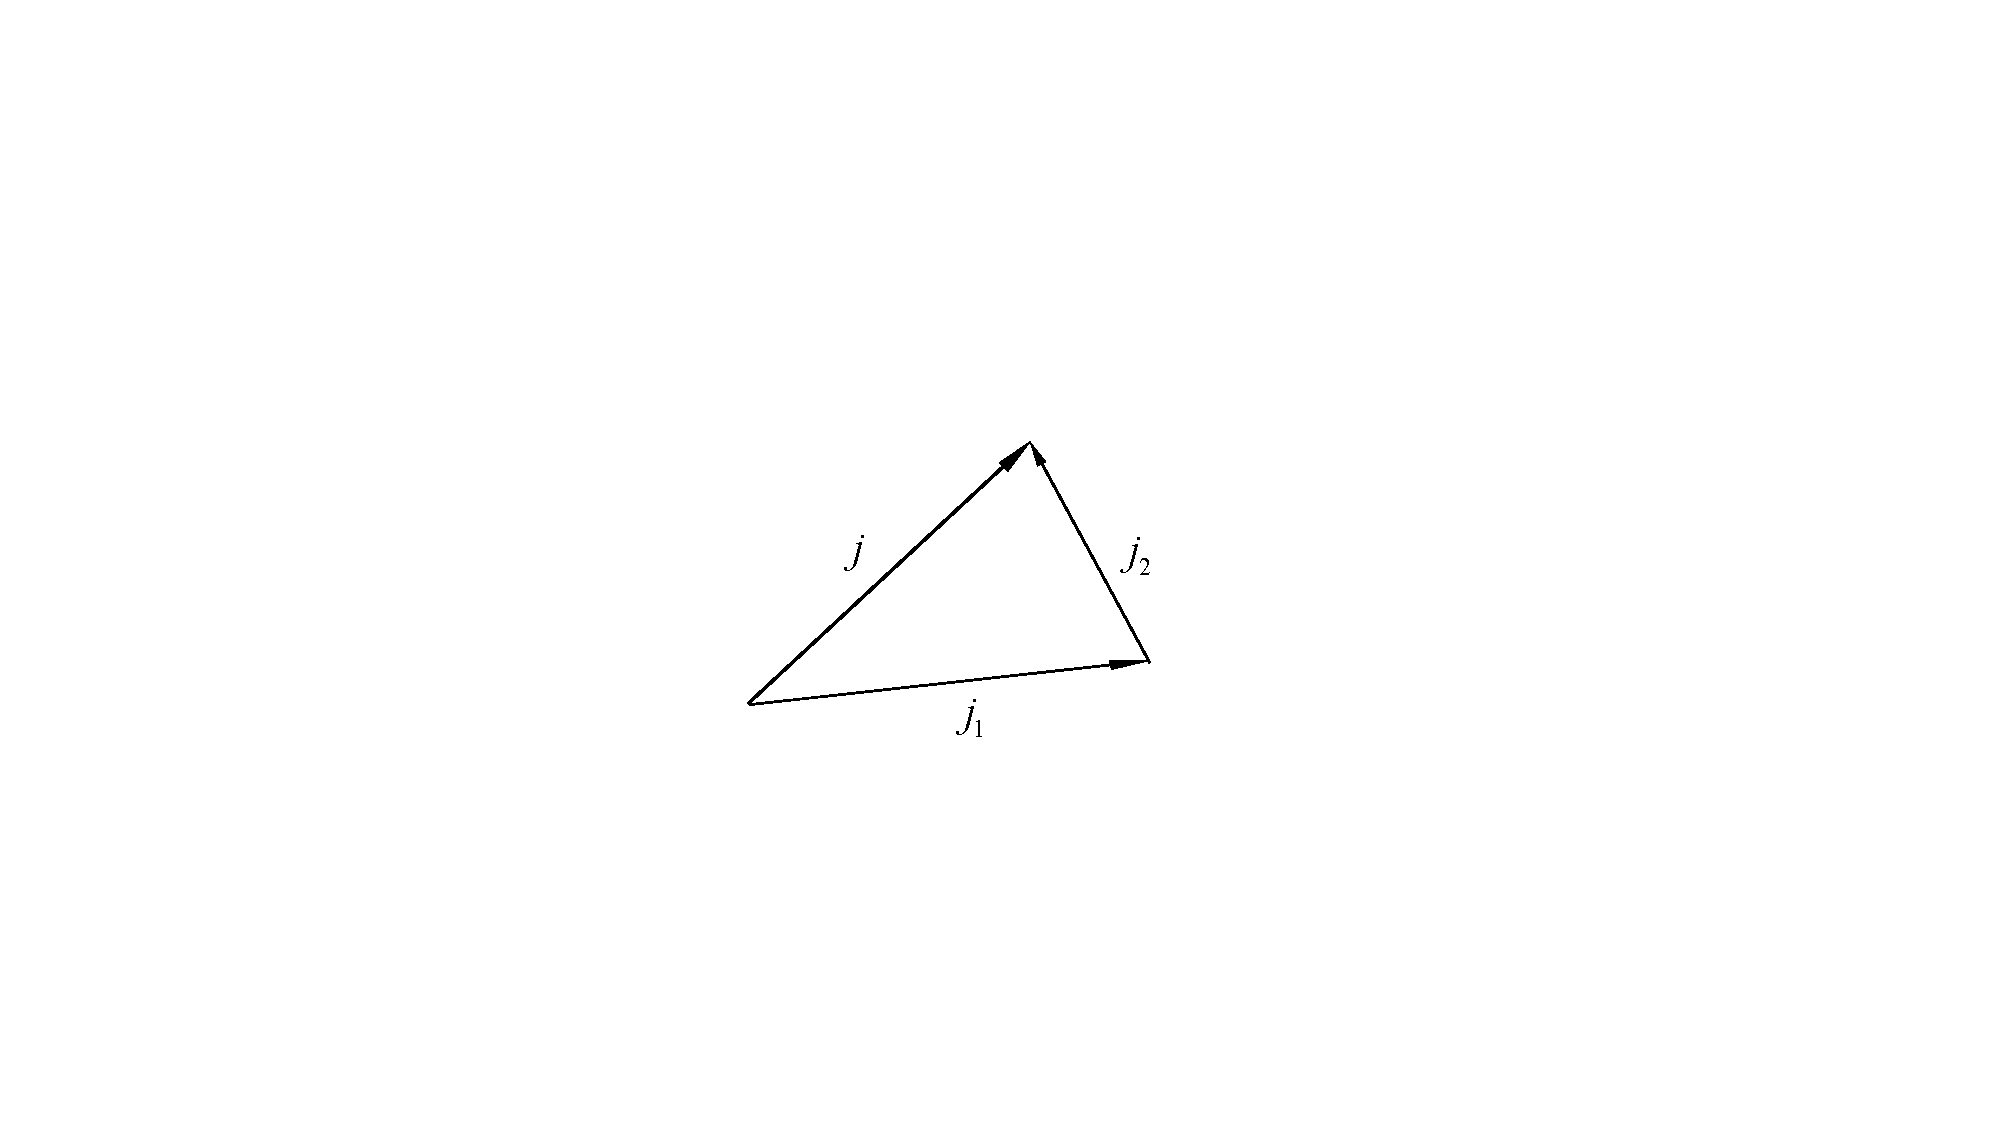
\includegraphics[width=3cm,clip]{QM file/figure/7-4}
	\caption{}\label{fig.7-4}
\end{wrapfigure}

\eqref{eq77.14}式中的系数$C(j,M,m_{1},m_{2})$称为C.G.(Clebsch-Gordan)系数,也称矢耦系数,有关理论和公式相当复杂,从略.如采用狄拉克态矢量符号,$\varPsi_{j_{1}m_{1}},\varPsi_{j_{2}m_{2}}$记成$|j_{1}m_{1},j_{2}m_{2}\rangle$,$\varPsi_{j_{1}j_{2}jM}$记成$|j_{1}j_{2}jM\rangle$,简写成$|jM\rangle$.给定$j_{1},j_{2}$后,我们就有一个$(2j_{1}+1)(2j_{2}+1)$维态矢量空间.如以$|j_{1}m_{1},j_{2}m_{2}\rangle$作为基矢,相应的表象称为非耦合表象;如以$|jM\rangle$作为基矢,相应的表象称为耦合表象.利用恒等变换公式
\begin{empheq}{equation}\label{eq77.17}
	\sum_{m_{1}}\sum_{m_{2}}|j_{1}m_{1},j_{2}m_{2}\rangle \langle j_{1}m_{1},j_{2}m_{2}|=1
\end{empheq}
将$|jM\rangle$在非耦合表象中展开成
\begin{empheq}{equation}\label{eq77.18}
	|jM\rangle=\sum_{m_{1}}\sum_{m_{2}}|j_{1}m_{1},j_{2}m_{2}\rangle \langle j_{1}m_{1},j_{2}m_{2}|jM\rangle 
\end{empheq}
与\eqref{eq77.14}式比较,易见
\begin{empheq}{equation}\label{eq77.19}
	C(jM,m_{1}m_{2})=\langle j_{1}m_{1}j_{2}m_{2}|jM \rangle 
\end{empheq}
显然C.G.系数就是联系两种表象的么正矩阵的矩阵元.

C.G.系数应用极广,有许多类型的C.G.系数表可供查阅.$j_{2}=\frac{1}{2}$和1时C.G.系数如表\ref{lab.7-1},表\ref{lab.7-2}所示.请将$\S$\ref{sec:07.02}中结果与表\ref{lab.7-1}对照$\bigg(j_{1}=l,j_{2}=\frac{1}{2},M=m+\frac{1}{2}\bigg)$


\begin{table}[!h]
	\begin{center}
		\caption{C.G.系数$\langle j_{1}m_{1}j_{2}m_{2}|jM\rangle\bigg(j_{2}=\dfrac{1}{2},m_{1}=M-m_{2}\bigg)$}
		\label{lab.7-1}
		\setlength{\tabcolsep}{8mm}	% 调节表格尺寸
		%\resizebox{h-length}{v-length}{text}
		\begin{tabular}{c|c|c}
			\toprule[1pt]
			\multirow{2}{*}{	} & \multirow{2}{*}{$m_{2}=\frac{1}{2}$} & \multirow{2}{*}{$m_{2}=-\frac{1}{2}$}	\\ 
			 & & \\
			\hline
			\multirow{2}{*}{}
			\multirow{2}{*}{$j=j_{1}+\frac{1}{2}$} & \multirow{2}{*}{$\sqrt{\frac{j_{1}+M+\frac{1}{2}}{2j_{1}+1}}$} & \multirow{2}{*}{$\sqrt{\frac{j_{1}-M+\frac{1}{2}}{2j_{1}+1}}$}	\\ 
			& & \\
			\hline
			\multirow{2}{*}{$j=j_{1}-\frac{1}{2}$} & \multirow{2}{*}{$-\sqrt{\frac{j_{1}-M+\frac{1}{2}}{2j_{1}+1}}$} & \multirow{2}{*}{$\sqrt{\frac{j_{1}+M+\frac{1}{2}}{2j_{1}+1}}$}	\\ 
			& & \\
			\bottomrule[1pt]
		\end{tabular}
	\end{center}
\end{table}

\begin{table}[!h]
	\begin{center}
		\caption{C.G.系数$\langle j_{1}m_{1}j_{2}m_{2}|jM\rangle\bigg(j_{2}=1,m_{1}=M-m_{2}\bigg)$}
		\label{lab.7-2}
		%\setlength{\tabcolsep}{3mm}	% 调节表格尺寸
		%\resizebox{h-length}{v-length}{text}
		\begin{tabular}{c|c|c|c}
			\toprule[1pt]
			\multirow{2}{*}{	}& \multirow{2}{*}{$m_{2}=1$} & \multirow{2}{*}{$m_{2}=0$} & \multirow{2}{*}{$m_{2}=-1$}	\\
			 & & & \\
			\hline
			\multirow{2}{*}{$j=j_{1}+1$} & \multirow{2}{*}{$\sqrt{\frac{(j_{1}+M)(j_{1}+M+1)}{(2j_{1}+1)(2j_{1}+2)}}$} & \multirow{2}{*}{$\sqrt{\frac{(j_{1}-M+1)(j_{1}+M+1)}{(j_{1}+1)(2j_{1}+1)}}$} 	& \multirow{2}{*}{$\sqrt{\frac{(j_{1}-M)(j_{1}-M+1)}{(2j_{1}+1)(2j_{1}+2)}}$}	\\
			 & & & \\
			\hline
			\multirow{2}{*}{$j=j_{1}$} & \multirow{2}{*}{$-\sqrt{\frac{(j_{1}+M)(j_{1}-M+1)}{2j_{1}(j_{1}+1)}}$} & \multirow{2}{*}{$\sqrt{\frac{M}{j_{1}(j_{1}+1)}}$} 	& \multirow{2}{*}{$\sqrt{\frac{(j_{1}-M)(j_{1}+M+1)}{2j_{1}(j_{1}+1)}}$}	\\
			 & & & \\
			\hline
			\multirow{2}{*}{$j=j_{1}-1$} & \multirow{2}{*}{$\sqrt{\frac{(j_{1}-M)(j_{1}-M+1)}{2j_{1}(2j_{1}+1)}}$} & \multirow{2}{*}{$-\sqrt{\frac{(j_{1}-M)(j_{1}+M)}{j_{1}(2j_{1}+1)}}$} 	& \multirow{2}{*}{$\sqrt{\frac{(j_{1}+M+1)(j_{1}+M)}{2j_{1}(2j_{1}+1)}}$}	\\
			 & & & \\
			\bottomrule[1pt]
		\end{tabular}
	\end{center}
\end{table}

\newpage







% 二电子体系的自旋波函数
\section[二电子体系的自旋波函数]{二电子体系的自旋波函数} \label{sec:07.08} % 


以$\boldsymbol{S}_{1}$和$\boldsymbol{S}_{2}$表示电子1和2的自旋角动量,体系的总自旋为
\eqshort
\begin{empheq}{equation}\label{eq78.1}
	\boldsymbol{S}=\boldsymbol{S}_{1}+\boldsymbol{S}_{2}
\end{empheq}
其分量为
\begin{empheq}{equation}\label{eq78.2}
	S_{z}=S_{1z}+S_{2z}
\end{empheq}\eqnormal
等等总自旋平方为
\begin{empheq}{equation}\label{eq78.3}
	\boldsymbol{S}^{2}=\boldsymbol{S}_{1}^{2}+\boldsymbol{S}_{2}^{2}+2\boldsymbol{S}_{1}\cdot\boldsymbol{S}_{2}
\end{empheq}
根据实验事实,
\eqshort
\begin{empheq}{equation}\label{eq78.4}
	\boldsymbol{S}_{1}^{2}=\boldsymbol{S}_{2}^{2}=\frac{3}{4}\hbar^{2}
\end{empheq}\eqnormal
这相当于$j_{1}=j_{2}=\frac{1}{2}$的情形.$\boldsymbol{S}^{2}$及$S_{z}$的本征值记为
\begin{empheq}{equation*}
	\boldsymbol{S}^{2}——S(S+1)\hbar^{2},\quad S_{z}--M_{s}\hbar
\end{empheq}
按照角动量耦合理论,总自旋量子数$S$的可能取值为1和0,$M_{s}$的取值为
\begin{empheq}{equation}\label{eq78.5}
	\boxed{\begin{aligned}
		S=1, &&M_{s}=1,0,-1	\\
		S=0, &&M_{s}=0
	\end{aligned}}
\end{empheq}
现在还需要确定$\boldsymbol{S}^{2},S_{z}$的共同本征态.

电子$1,2$各有两种独立自旋态$\chi_{1/2}$,$\chi_{-1/2}$,在这里记为$\alpha,\beta$.非耦合表象中的基矢$|j_{1}m_{1},j_{2}m_{2}\rangle$共有4个,它们是
\begin{empheq}{equation}\label{eq78.6}
	\alpha(1)\alpha(2),\alpha(1)\beta(2),\beta(1)\alpha(2),\beta(1)\beta(2)
\end{empheq}
它们都是总$S_{z}$的本征态,$M_{s}$依次为$1,0,0,-1$.按照\eqref{eq78.5}式,$M_{s}$等于1和-1时,$S$必然为1.因此可以判断$\alpha(1)\alpha(2)$和$\beta(1)\beta(2)$都已经是$\boldsymbol{S}^{2},S_{z}$的共同本征态$|S,M_{S}\rangle$,在这里记成$\chi_{SM_{S}}$,即
\begin{empheq}{equation}\label{eq78.7}
	\chi_{11}=\alpha(1)\alpha(2),\quad \chi_{1-1}=\beta(1)\beta(2)
\end{empheq}
$S=1$时,$\boldsymbol{S}^{2},S_{z}$还有一个共同本征态$(M_{S}=0)$,它应该由\eqref{eq78.6}式中第二、三项叠加而成.按照角动量一般理论[\eqref{eq47.26}式]
\begin{empheq}{equation}\label{eq78.8}
	(S_{x}-iS_{y})\chi_{11}=\sqrt{2}\hbar\chi_{10}
\end{empheq}
其中$(S_{x}-iS_{y})=(S_{1x}-iS_{1y})+(S_{2x}-iS_{2y})$.利用\eqref{eq71.19}式容易算出
\begin{empheq}{equation*}
	(S_{x}-iS_{y})\chi_{11}=\hbar\alpha(1)\beta(2)+\hbar\beta(1)\alpha(2)
\end{empheq}
代入\eqref{eq78.8}式,即得
\begin{empheq}{equation}\label{eq78.9}
	\chi_{10}=\frac{1}{\sqrt{2}}[\alpha(1)\beta(2)+\beta(1)\alpha(2)]
\end{empheq}
按照角动量一般理论,$\chi_{10}$与$\chi_{1-1}$有关系
\begin{empheq}{equation}\label{eq78.10}
	(S_{x}-iS_{y})\chi_{10}=\sqrt{2}\hbar\chi_{1-1}
\end{empheq}
请读者自行验证.

$\boldsymbol{S}^{2},S_{z}$还有一个共同本征态$\chi_{00}(S=0,M_{S}=0)$,它应该由\eqref{eq78.6}式中第二、三项叠加而成,并与$\chi_{10}$正交(因为量子数$S$之值不同),设
\begin{empheq}{equation*}
	\chi_{00}=C_{1}\alpha(1)\beta(2)+C_{2}\beta(1)\alpha(2)
\end{empheq}
由正交条件
\eqshort
\begin{empheq}{equation*}
	\chi_{10}^{+}\chi_{00}=0
\end{empheq}\eqnormal
容易得出$C_{2}=-C_{1}$.取$C_{1}>0$.并将$\chi_{00}$归一化,最后得到
\begin{empheq}{equation}\label{eq78.11}
	\chi_{00}=\frac{1}{\sqrt{2}}[\alpha(1)\beta(2)-\beta(1)\alpha(2)]
\end{empheq}
利用\eqref{eq71.17}式容易验证$S_{\chi_{00}},S_{\chi_{00}}^{2}=0$.

总结以上计算,我们已经求出二电子体系总自旋平方$\boldsymbol{S}^{2}$和$S_{z}$的全部共同本征函数$\chi_{SM_{S}}$,它们是
\begin{empheq}{equation}\label{eq78.12}
	\begin{aligned}
		\chi_{11} &=\alpha(1)\alpha(2)	\\
		\chi_{10} &=\frac{1}{\sqrt{2}}[\alpha(1)\beta(2)+\beta(1)\alpha(2)]	\\
		\chi_{1-1}&=\beta(1)\beta(2)	\\
		\chi_{00} &=\frac{1}{\sqrt{2}}[\alpha(1)\beta(2)-\beta(1)\alpha(2)]
	\end{aligned}
\end{empheq}
容易验证,它们和表\ref{lab.7-1}列出的C.G.系数是一致的.\eqref{eq78.12}式适用于任何由两个自旋$\frac{1}{2}$粒子组成的体系,应用极广,读者应该牢记.

作为二粒子体系自旋自由度的波函数,\eqref{eq78.6}式4个波函数都能够表示成单粒子波函数的乘积,称为“分离态”.反之,\eqref{eq78.9}式和\eqref{eq78.11}式则为“纠缠态”.近年来由于量子信息论的迅速发展,纠缠态日益引人注目.对于本节讨论的自旋波函数,典型的纠缠态除$\chi_{10}$、$\chi_{00}$外,还有
\begin{empheq}{equation}\label{eq78.13}
	\frac{1}{\sqrt{2}}[\alpha(1)\alpha(2)\pm\beta(1)\beta(2)]
\end{empheq}
它们都是$\sigma_{1x},\sigma_{2x},\sigma_{1z},\sigma_{2z}$的共同本征函数.








% 习题
\begin{exercises}
	
\exercise $n\times n$矩阵$M$的“迹”定义为$\tr M=\sum_{k=1}^{n}M_{kk}$,即对角矩阵元之和证明:任意2阶矩阵$M$可以表示成泡利矩阵$\sigma_{x},\sigma_{y},\sigma_{z}$与单位矩阵$I$的线性叠加,如下式:
\eqlong
\begin{empheq}{align*}
	M &=\frac{1}{2}(\tr M)I+\frac{1}{2}(\tr\boldsymbol{\sigma}M)\cdot\boldsymbol{\sigma}	\\
	&= \frac{1}{2} \{(\tr M)I+(\tr\sigma_{x}M)\sigma_{x}+(\tr\sigma_{y}M)\sigma_{y}+(\tr\sigma_{z}M)\sigma_{z}\}
\end{empheq}\eqnormal
 
\exercise 在$S_{z}$表象中,求$\sigma_{x}$的本征函数及$\sigma_{y}$的本征函数.
 	
\exercise 在$S_{z}$表象中,求$\sigma_{n}$的矩阵表示及其本征函数.$\sigma_{n}=\boldsymbol{n}\cdot\boldsymbol{\sigma}$,$\boldsymbol{n}$为任意$(\theta,\varphi)$方向单位矢量.
 	
\exercise 对于上题求得两个$\sigma_{n}$本征函数,计算$\langle\boldsymbol{\sigma}\rangle$,并求$\Delta S_{x},\Delta S_{y},\Delta S_{z}$,验证不确定关系.
 	
\exercise 证明$(\sigma_{x}+i\sigma_{y})^{2}=0,(\sigma_{x}-i\sigma_{y})^{2}=0$.用$(\sigma_{x}\pm i\sigma_{y})$的矩阵表示($S_{z}$表象)验证这两个公式.
 	
\exercise 讨论下列算符是否存在.如存在,将其表示成$I,\sigma_{x},\sigma_{y},\sigma_{z}$的线性叠加.

(a)$(1+\sigma_{x})^{\frac{1}{2}}$\quad(b)$(1+\sigma_{x}+i\sigma_{y})^{\frac{1}{2}}$\quad (c)$(1+\sigma_{z})^{-1}$
 
\exercise 证明公式$e^{i\lambda\sigma_{z}}=\cos\lambda+i\sigma_{z}\sin\lambda$.($\lambda$为实参数,$\sigma_{z}$为算符)并在$S_{z}$表象中证明
\begin{empheq}{equation*}
	e^{i\lambda\sigma_{z}}=\begin{bmatrix}
		e^{i\lambda} & 0 	\\
		0 & e^{-i\lambda}	\\
	\end{bmatrix}
\end{empheq}
 
\exercise 设$\boldsymbol{A}$为常数矢量,令$\boldsymbol{A}\cdot\boldsymbol{\sigma}=A\sigma_{A}$.证明
\begin{empheq}{equation*}
	e^{i\boldsymbol{A}\cdot\boldsymbol{\sigma}}=\cos A+i\sigma_{A}\sin A
\end{empheq}
 	
\exercise 设$\boldsymbol{A},\boldsymbol{B},\boldsymbol{C}$为常数矢量,求$\tr(\boldsymbol{A}\cdot\boldsymbol{\sigma}),\tr[(\boldsymbol{A}\cdot\boldsymbol{\sigma})(\boldsymbol{B}\cdot\boldsymbol{\sigma})]$及$\tr[(\boldsymbol{A}\cdot\boldsymbol{\sigma})(\boldsymbol{B}\cdot\boldsymbol{\sigma})(\boldsymbol{C}\cdot\boldsymbol{\sigma})]$.
 	
\exercise 证明$\tr(e^{i\boldsymbol{A}\cdot\boldsymbol{\sigma}})=2\cos A$,$\tr(e^{i\lambda\sigma_{x}} e^{i\lambda\sigma_{y}}=2\cos^{2}A)$.
 	
\exercise 证明(a) $\sigma_{z}(\sigma_{x}\pm i\sigma_{y})=(\sigma_{x}\pm i\sigma_{y})(\sigma_{z}\pm 2)$

(b) $f(\sigma_{z})(\sigma_{x}\pm i\sigma_{y})=(\sigma_{x}\pm i\sigma_{y})f(\sigma_{z}\pm 2)$

(c) $e^{i\lambda\sigma_{z}}(\sigma_{x}\pm i\sigma_{y})=e^{\pm2i\lambda}(\sigma_{x}\pm i\sigma_{y})e^{i\lambda\sigma_{z}}$
 	
\exercise 证明$e^{i\lambda\sigma_{z}}\sigma_{x}e^{-i\lambda\sigma_{z}}=\sigma_{x}\cos2\lambda-\sigma_{y}\sin2\lambda$

$e^{i\lambda\sigma_{z}}\sigma_{y}e^{-i\lambda\sigma_{z}}=\sigma_{x}\sin2\lambda+\sigma_{y}\cos2\lambda$
 	
\exercise 令$\hbar=1$,对于电子,证明
\eqlong
\begin{empheq}{equation*}
	(2\boldsymbol{S}\cdot\boldsymbol{L}+1)^{2}=\boldsymbol{J}^{2}+\frac{1}{4},\quad (\boldsymbol{\sigma}\cdot\boldsymbol{J})(\boldsymbol{\sigma}\cdot\boldsymbol{J}-1)=\boldsymbol{J}^{2}
\end{empheq}\eqnormal
 	
\exercise 对于电子的$(\boldsymbol{L}^{2},\boldsymbol{J}^{2},J_{z})$共同本征态$\varPsi_{ljm_{j}}$,对于属于同一个$l$值的那些状态,定义算符
\begin{empheq}{equation*}
	\Lambda_{l}^{+}=\frac{1}{2l+1}(l+1+\boldsymbol{\sigma}\cdot\boldsymbol{L}),\quad \Lambda_{l}^{-}=\frac{1}{2l+1}(l-\boldsymbol{\sigma}\cdot\boldsymbol{L})
\end{empheq}
试确定它们对$\varPsi_{ljm_{j}}$的作用规则,并找出它们满足的基本代数关系.
 	
\exercise  (a) 证明$\sigma_{r}=\dfrac{\boldsymbol{\sigma}\cdot\boldsymbol{r}}{r}$与$\boldsymbol{J}$的各分量对易,即$[\sigma_{r},\boldsymbol{J}]=0$

(b) 对于$\varPsi_{ljm_{j}}$,将$l=j-\dfrac{1}{2}$者记为$\phi_{jm_{j}}^{A}$,$l=j+\dfrac{1}{2}$者记为$\phi_{jm_{j}}^{B}$,证明
\begin{empheq}{equation*}
	\sigma_{r}\phi_{jm_{j}}^{A}=-\phi_{jm_{j}}^{B},\quad \sigma_{r}\phi_{jm_{j}}^{B}=-\phi_{jm_{j}}^{A}
\end{empheq}
并加以解释.

[提示:利用附录\ref{A04}\eqref{eqA4.45}式、\eqref{eqA4.46}式,并注意问题的宇称性]

 	
\exercise 电子的总磁矩算符是
\begin{empheq}{equation*}
	\boldsymbol{\mu}=\boldsymbol{\mu}_{L}+\boldsymbol{\mu}_{s}=-\dfrac{e}{2m_{e}c}(\boldsymbol{L}+2\boldsymbol{S})
\end{empheq}
试对于$\varPsi_{ljj}$态$(m_{j}=j)$计算$\mu_{z}$平均值(结果用量子数$j$表示).
 
\exercise 某电子态波函数为$\Psi(r,\theta,\varphi,S_{z})=R(r)Y_{l0}(\theta,\varphi)\chi_{1/2}(S_{z})$.这是否$\boldsymbol{J}^{2}$或$J_{z}$本征函数?试计算$\langle\boldsymbol{J}^{2}\rangle$,从而求出$\boldsymbol{J}^{2}$的可能测值及相应概率.
 	
\exercise 自旋为0的带电粒子在均匀磁场中运动,哈密顿算符为
\begin{empheq}{equation*}
	\hat{H}=\frac{m}{2}\hat{\boldsymbol{v}}^{2}=\frac{1}{2m}\bigg(\hat{\boldsymbol{p}}-\frac{q}{c}\boldsymbol{A}\bigg)^{2}
\end{empheq}

设磁场沿$z$轴方向,矢势取为$\boldsymbol{A}=\dfrac{1}{2}\boldsymbol{B}\times\boldsymbol{r}$,即
\begin{empheq}{equation*}
	A_{x}=-\frac{By}{2},\quad A_{y}=\frac{Bx}{2},\quad A_{z}=0
\end{empheq}

(a) 计算$v_{x},v_{y},v_{z}$之间的对易式

(b) 设粒子电荷$q>0$.证明$\hat{H}$可以表示成
\begin{empheq}{equation*}
	\hat{H}=\frac{\hbar qB}{2mc}(\hat{Q}^{2}+\hat{P}^{2})+\frac{1}{2m}\hat{p}_{z}^{2}
\end{empheq}
确定$\hat{Q},\hat{P}$,证明$\hat{Q}\hat{P}-\hat{P}\hat{Q}$.

(c) 利用谐振子的结果,确定本题的能谱.
 	
\exercise 将上题的$\hat{H}$表示成\eqref{eq74.7'}式的形式,找出主要的守恒力学量,再找出能级公式.(质量$m$改为$\mu$,以免与量子数混淆.)
 	
\exercise 有一个定域电子(不考虑“轨道”运动),受到沿正$x$方向的均匀磁场作用,磁作用势为
\begin{empheq}{equation*}
	H=\frac{eB}{m_{e}c}S_{x}=\frac{e\hbar B}{2m_{e}c}\sigma_{x}
\end{empheq}
设$t=0$时电子的自旋状态为$\sigma_{z}=1$的本征态,即$\chi_{1/2}=\left[\begin{smallmatrix}
	1 \\ 0 
\end{smallmatrix}\right]$.求任意$t>0$时自旋波函数$\chi(t)=\left[\begin{matrix}
	a(t)	\\	b(t)
\end{matrix}\right]$,并求$\overline{S_{x}}(t),\overline{S_{y}}(t),\overline{S_{z}}(t)$.
 
\exercise 用海森伯运动方程处理上题,求$\overline{S_{x}}(t),\overline{S_{y}}(t),\overline{S_{z}}(t)$.注意先确定$t=0$时它们的初始值.
 	
\exercise 对于氢原子,求自旋轨道耦合作用引起的能级分裂$\Delta E_{nl}$[\eqref{eq73.15}式、\eqref{eq73.12}式]

[提示:$\langle r^{-3}\rangle$利用5-15题结果.]
 
\exercise 设氢原子中电子处于s态$(l=0)$,考虑电子与质子的自旋角动量,$S_{1}$与$S_{2}$.设电子自旋态为$\alpha$,质子自旋态为$\beta$,即总自旋态为$\alpha(1)\beta(2)$.求总自旋平方$\boldsymbol{S}^{2}=(\boldsymbol{S}_{1}+\boldsymbol{S}_{2})^{2}$的可能取值及相应概率.
 	
\exercise 同上题,如电子处于$S_{1z}=\dfrac{\hbar}{2}$的状态(即$\chi_{1/2}$),质子处于$S_{2x}=\dfrac{\hbar}{2}$的状态,求总自旋平方$\boldsymbol{S}^{2}$及总$S_{z}=S_{1z}+S_{2z}$的可能取值及相应概率.
 	
\exercise 考虑由3个自旋$\dfrac{1}{2}$的可分辨粒子组成的体系.

(a) 求总自旋平方$\boldsymbol{S}^{2}=(\boldsymbol{S}_{1}+\boldsymbol{S}_{2}+\boldsymbol{S}_{3})^{2}$的本征值.

(b) 设体系能量算符(略去“轨道”运动)为
\begin{empheq}{equation*}
	H=(\boldsymbol{S}_{1}\cdot\boldsymbol{S}_{2}+\boldsymbol{S}_{2}\cdot\boldsymbol{S}_{3}+\boldsymbol{S}_{3}\cdot\boldsymbol{S}_{1})\omega_{0}
\end{empheq}
求能谱,并说明各能级的简并度.
 	
\exercise 两个角动量耦合问题,设$j_{1}=j_{2}=1$,则$m_{1}$及$m_{2}$均有1,0,-1三种取值,相应的本征态记为$\alpha,\beta,\gamma$,$|j_{1}=1,m_{1}=1\rangle$记为$\alpha(1)$,$|j_{2}=1,m_{2}=0\rangle$记为$\beta(2)$,依此类推.$\boldsymbol{J}_{1}^{2},\boldsymbol{J}_{2}^{2},\boldsymbol{J}^{2},J_{z}$共同本征态记为$\varPsi_{jM}$.对于本题$(j_{1}=j_{2}=1)$,共有多少种$\varPsi_{jM}$?将它们在无耦合表象中求出来.(计算时,取$\hbar=1$.)

[ 提示:利用$J_{1+}\gamma(1)=\sqrt{2}\beta(1),J_{1+}\beta(1)=\sqrt{2}\alpha(1),J_{1+}\alpha(1)=0$,等等.$\boldsymbol{J}^{2}=\boldsymbol{J}_{1}^{2}+\boldsymbol{J}_{2}^{2}+2\boldsymbol{J}_{1z}\boldsymbol{J}_{2z}+J_{1+}J_{2-}+J_{1-}J_{2+},\boldsymbol{J}_{1}^{2}=\boldsymbol{J}_{2}^{2}=2$.]
 	
\exercise 对于二电子体系的自旋三重态和单态$(\chi_{00})$,证明它们都是$\boldsymbol{\sigma_{1}}\cdot\boldsymbol{\sigma_{2}}$的本征态,本征值分别为1和-3.
 
\exercise 同上题,验证$\chi_{00}$是$\sigma_{1x}\sigma_{2x},\sigma_{1y}\sigma_{2y},\sigma_{1z}\sigma_{2z}$的共同本征态,本征值均为-1.
 	
\exercise 对于自旋单态$\chi_{00}$,求$(\boldsymbol{a}\cdot\boldsymbol{\sigma_{1}})(\boldsymbol{b}\cdot\boldsymbol{\sigma_{2}})$的平均值.其中$\boldsymbol{a},\boldsymbol{b}$为常矢量.

\exercise 对于自旋单态和三重态$\chi_{00},\chi_{11},\chi_{10},\chi_{1-1}$,找出使它们互相转化的算符(共12种)建议不要用角动量升降算符,而用尽量简单的、存在逆算符的单体或二体算符.
	
\end{exercises}
